% Material found at https://www.elsevier.com/authors/author-schemas/latex-instructions

\documentclass{elsarticle}

\usepackage{lineno,hyperref}
\modulolinenumbers[5]

%=== Added for MU paper ====
\usepackage{color,soul} %% this was needed to have highlighted text
\usepackage{graphicx}
\usepackage{array,colortbl,xcolor}
\usepackage{hyperref}
\usepackage{amsmath}
\usepackage{amssymb}
\usepackage{mathtools}
\usepackage{nomencl}
\usepackage{bm}
\usepackage{subcaption}
\usepackage{systeme}
\makenomenclature

\graphicspath{{./figures/}}

\renewcommand{\labelenumii}{\theenumii}
\renewcommand{\theenumii}{\theenumi.\arabic{enumii}.}

\journal{Reliability Engineering \& System Safety}

%%%%%%%%%%%%%%%%%%%%%%%
%% Elsevier bibliography styles
%%%%%%%%%%%%%%%%%%%%%%%
%% To change the style, put a % in front of the second line of the current style and
%% remove the % from the second line of the style you would like to use.
%%%%%%%%%%%%%%%%%%%%%%%

%% Numbered
\bibliographystyle{model1-num-names}

%% Numbered without titles
%\bibliographystyle{model1a-num-names}

%% Harvard
%\bibliographystyle{model2-names.bst}\biboptions{authoryear}

%% Vancouver numbered
%\usepackage{numcompress}\bibliographystyle{model3-num-names}

%% Vancouver name/year
%\usepackage{numcompress}\bibliographystyle{model4-names}\biboptions{authoryear}

%% APA style
%\bibliographystyle{model5-names}\biboptions{authoryear}

%% AMA style
%\usepackage{numcompress}\bibliographystyle{model6-num-names}

%% `Elsevier LaTeX' style
%\bibliographystyle{elsarticle-num}
%%%%%%%%%%%%%%%%%%%%%%%

\begin{document}

\begin{frontmatter}

\title{Measuring Risk-Importance in a Simulation-Based PRA Framework - 
       Part I: Mathematical Framework}
%% \tnotetext[mytitlenote]{Fully documented templates are available in the elsarticle package on \href{http://www.ctan.org/tex-archive/macros/latex/contrib/elsarticle}{CTAN}.}

%% Group authors per affiliation:
\author{D. Mandelli, Z. Ma, C. Parisi, D. Maljovec, A. Alfonsi, C. Smith}
\address{Idaho National Laboratory (INL), 2525 Fremont Ave, 83402 Idaho Falls (ID), USA}

\begin{abstract}
  Risk importance measures are indexes that are used to rank systems, 
structures and components (SSCs) using risk-informed methods. 
The most used/known measures are: Risk Reduction Worth (RRW), 
Risk Achievement Worth (RAW), Birnbaum (B) and Fussell-Vesely (FV). 
Once obtained from classical Probabilistic Risk Analysis (PRA) analyses, 
these risk measures can be effectively employed to relatively rank
component importance.
In contrast to classical PRA methods, 
Dynamic PRA methods couple stochastic models with safety analysis 
codes to determine risk associate to complex systems such as nuclear 
plants. Compared to classical PRA methods, simulation-based approaches
can evaluate with 
higher resolution the safety impact of timing and sequencing of events 
on the accident progression. 
The objective of this paper is to present a series of methods that 
can be employed to measure risk importance of components which are 
part of complex systems such as nuclear power plants.
The first set of measures are directly derived from classical risk 
importance measures (e.g., RRW, RAW, B and FV) and that can be employed
to any Dynamic PRA analysis.
In addition, we provide a set of risk importance measures that capture the 
dynamic nature of the problem and provide insight related to plant safety 
margins.

\end{abstract}

\begin{keyword}
%% keywords here, in the form: keyword \sep keyword
Importance Measures \sep Dynamic PRA \sep Probabilistic Risk Assessment 
\end{keyword}

\end{frontmatter}

\linenumbers

\printnomenclature[1in]

\section{Introduction}
\label{sec:introduction}
RAVEN (\textbf{R}isk \textbf{A}nalysis \textbf{V}irtual \textbf{EN}vironment)~\cite{Nureg1150}  is one of the many INL-developed software tools researchers can 
use to identify and 
increase the safety margin in complex systems (e.g. Nuclear Power Plants). It is a modular or ``plug-able'' framework that can be coupled with other computer 
modeling systems. RAVEN is capable to agnostically communicate with any system 
code. This agnosticism includes providing Application Programming Interfaces (APIs). These APIs are used to allow RAVEN to interact with any code as long as all 
the parameters that need to be perturbed are accessible through input files or via python interfaces. 
As a generic software framework, RAVEN is designed to perform parametric and probabilistic analysis based on the response of complex system codes. RAVEN is 
capable of investigating the system response as well as the input space using standard sampling techniques (e.g Monte Carlo, Grid, or Latin Hyper Cube), but its 
strength is focused toward system feature discovery, such as limit surfaces (i.e. separating regions of the input space leading to system failure, using dynamic 
supervised learning techniques), and advanced data analysis methodologies (i.e. Topology-based domain decomposition, Data Mining, Clustering, etc.).

The development of RAVEN has begun in 2012 to satisfy the need to provide a modern risk evaluation framework. RAVEN principal assignment is to provide the 
necessary software and algorithms in order to employ the concept developed by the Risk Informed Safety Margin Characterization (RISMC) path-
way~\cite{RISMC}. 
RISMC is one of the pathways defined within the Light Water Reactor Sustainability (LWRS) program. In the RISMC approach, the goal is not just specifically 
identifying the frequency of an event potentially leading to a system failure, but also to analyze the ``distance'' and the drivers toward the happening of key 
safety-related events. This approach may be used in identifying and increasing the safety margins related to those events. A safety margin is a numerical value 
quantifying the probability that a safety metric (e.g. as peak pressure in a pipe) is exceeded under certain conditions. The initial development of RAVEN has 
been focused on providing dynamic risk assessment capability to RELAP-7~\cite{RELAP7}, currently under development at the INL. All the methodologies
developed have been modularized in order to be applied to any computer modeling system (e.g., BISON, RELAP-7, RELAP5-3D, MELCOR, etc.).

The aim of this manuscript is to present a peculiar capability within the RAVEN framework named \textit{``EnsembleModels''}.

RAVEN is currently able to construct multi-targets Reduced Order Models (Ref.4), which are aimed to represent the response of a system (in a 
fixed configuration) for multiple Figures of Merits (FOMs) and time-dependent ROMs (see Ref.5). These capabilities represent the initial steps for a larger 
implementation about the interaction of multiple models. In fact, in several cases, multiple models need to interface with each other since the initial conditions of 
one are dependent on the outcomes of another.
To better understand the problem that here is solved, it is useful to consider two simple examples:
\begin{enumerate}
  \item The following problem is considered: a weather forecast simulation code ``a'' is used to compute the external (i.e. ambient) temperature in a certain location. 
  A second model ``b'' is inquired to compute the average temperature in a room having as boundary condition, among several others, the external ambient 
  temperature. The response of the model ``b'' depends on the outcome of the model ``a'';
   \item Two different simulation codes are considered: a) a code that is meant to compute the thermal conductivity of the ceramic Uranium Dioxide (UO2) as 
   function of the Temperature, and b) a Thermal-hydraulic (TH) code that is used to compute the Temperature field of a reactor, whose heat conduction depends on 
   the thermal conductivity value. As easily inferable, the two models are mutual dependent, determining in a non-linear system of equations.
\end{enumerate}
The two reported examples are only aimed to illustrate the reason why the creation of a framework to make interact different models is a key development for the 
advancement of RAVEN as a comprehensive calculation flow driver. Before reporting how the ensemble-models have been implemented, it is necessary to briefly 
describe the representative Model ``entities'' that are available in RAVEN.



\begin{figure}
    \centering
    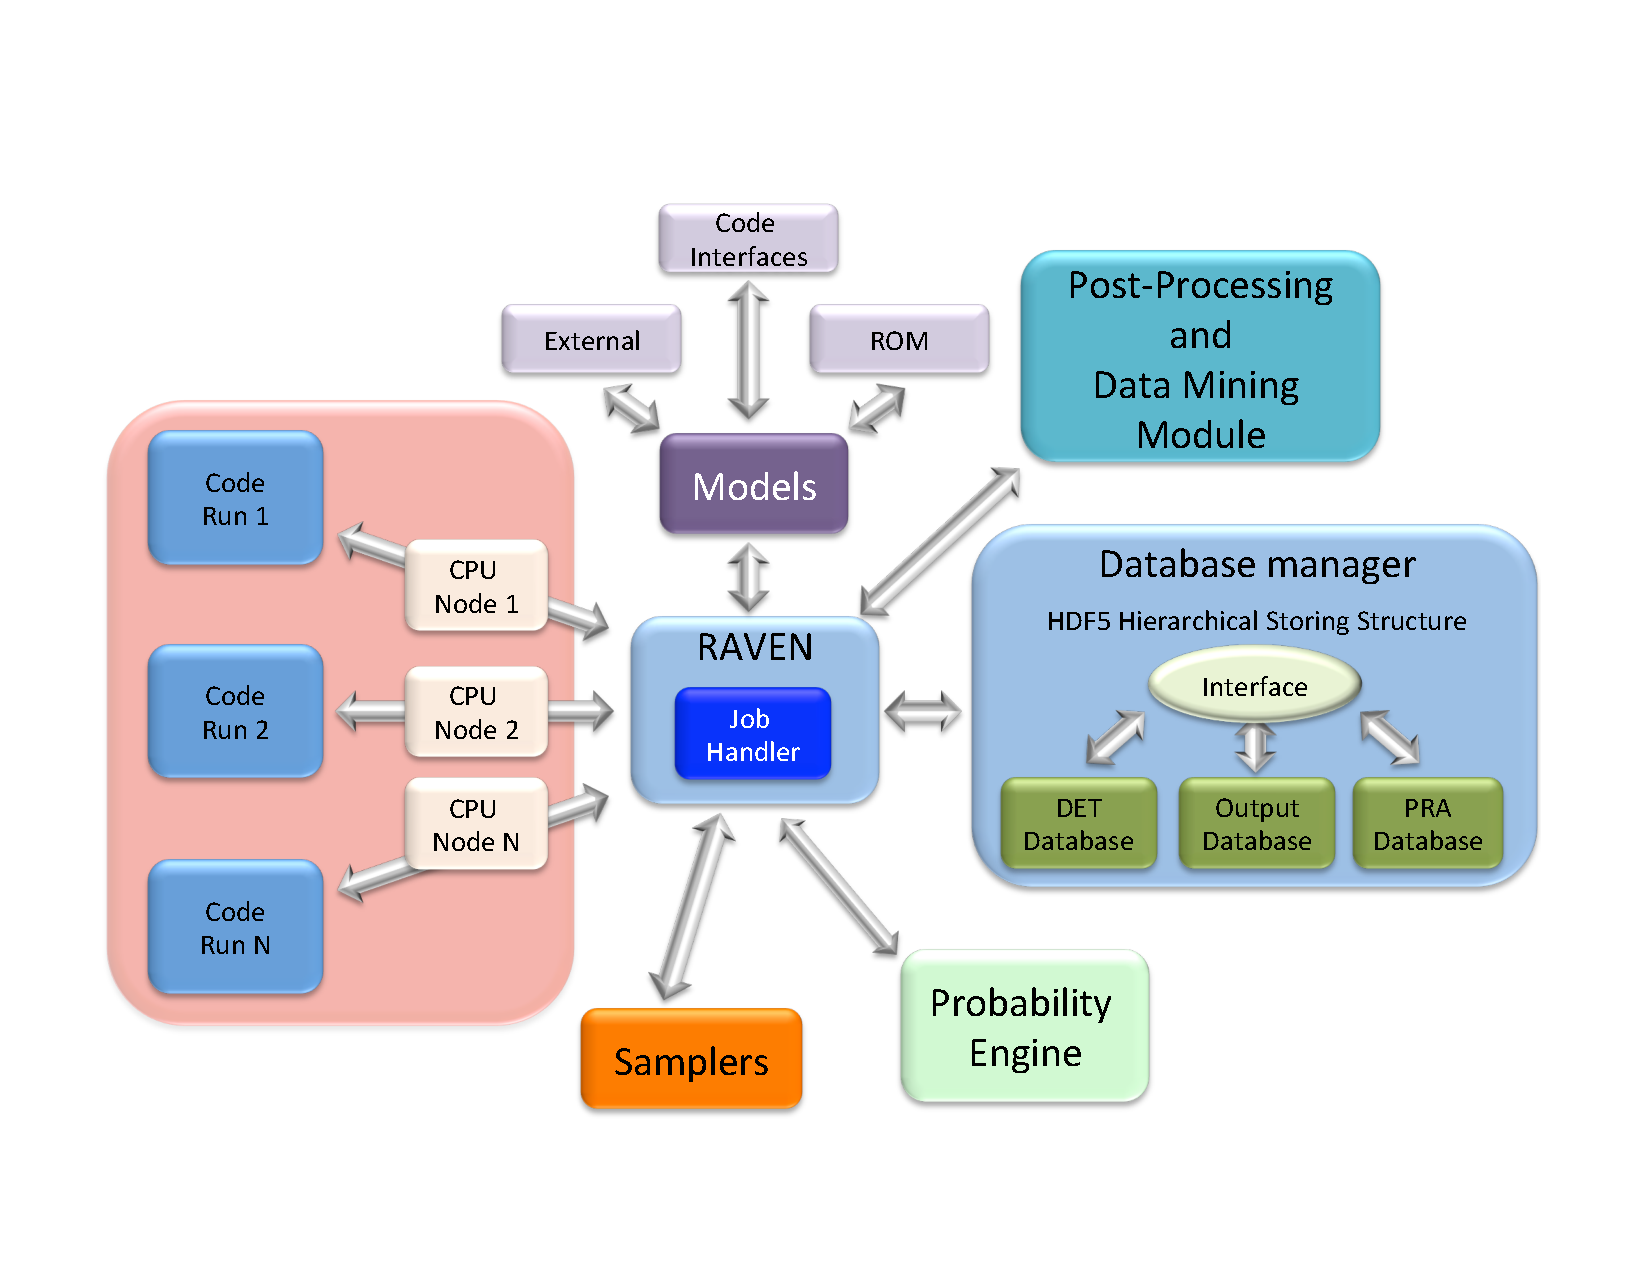
\includegraphics[scale=0.5]{raven.pdf}
    \caption{RAVEN}
    \label{fig:raven}
\end{figure}

\section{Classical RIMs}
\label{sec:classicalRIMs}

% In classical PRA methods, for any basic event, the most used RIMs measures are: 
% Risk Achievement Worth (RAW), Risk Reduction Worth (RRW), Birnbaum (B) and 
% Fussell-Vesely (FV)~\cite{flemingRiskImportance}. 
% All these RIMs are calculated by determining three values based on core damage 
% frequency (CDF):
% \begin{itemize}
%   \item $R_0$: nominal CDF
%   \item $R_i^-$: CDF for basic event i assuming perfectly reliable
%   \item $R_i^+$: CDF for basic event i assuming it has failed
% \end{itemize}
% 
% Once these three values are determined, then the RIMs are calculated~\cite{} as 
% follows for each basic event $i$:
% \begin{align} 
%   RAW_i &= \frac{R_i^+}{R_0}    \\
%   RRW_i &= \frac{R_0}{R_i^-}    \\
%   B_i &= R_i^+-R_i^-            \\
%   FV_i &= \frac{R_0-R_i^-}{R_0} 
% \end{align}
% 
% Note the four RIMs listed above is not exhaustive: in literature it is possible to 
% find additional RIMs such as the 
% Differential Importance Measure (DIM)~\cite{BorgonovoApostolakis}. 
% Since, the scope of this paper is tight to risk-informed application of 10CFR50.69, 
% we will focus this paper only on the four RIMs listed above.

Nuclear industry PRA codes such as SAPHIRE can calculate the following seven different basic event importance 
measures for each basic event for the respective fault tree, accident sequence, or end state:
\begin{itemize}
  \item Fussell-Vesely (FV)
  \item Risk Increase Ratio (RIR)
  \item Risk Increase Difference (RID)
  \item Risk Reduction Ratio (RRR)
  \item Risk Reduction Difference (RRD)
  \item Birnbaum (B)
  \item Uncertainty Importance
\end{itemize}   
  
The FV importance measure indicates the fraction of the minimal cut set upper bound 
(or sequence frequency, core damage frequency) contributed by the cut sets containing the basic event of interest. 
It is calculated in SAPHIRE Version 8 as $FV = F(i) / F(x)$
where:
\begin{itemize}
  \item $F(x)$ is the value of all the minimal cut sets evaluated with the basic event probabilities at their mean value
  \item $F(i)$ is the value of all the minimal cut sets that contain the basic event $i$.
\end{itemize}

    
The RIR or RID importance measure indicates the increase (in relative ratio changes or in actual differences) of the minimal cut set upper bound (or sequence frequency, core damage frequency) when the basic event of interest has failed (i.e., the basic event failure probability is 1.0). 

The RIR importance is often called Risk Achievement Worth (RAW) in industry. The risk increase importance measures are calculated in SAPHIRE Version 8 as follows: $RIR = F(1)/F(x)$ and $RID=F(1)-F(x)$
where:
\begin{itemize} 
  \item $F(x)$ is the value of all the minimal cut sets evaluated with the basic event probabilities at their mean value.
  \item $F(1)$ is the value of all the minimal cut sets evaluated with the probability of the basic event of interest set to 1.0.
\end{itemize}

The RRR or RRD importance measure indicates the reduction (in relative ratio changes or in actual differences) of the minimal cut set upper bound (or sequence frequency, core damage frequency) if the basic event of interest never fails (i.e., the basic event failure probability is 0.0). The Risk Reduction Ratio importance is also often called RRW in industry. The risk decrease importance measures are calculated in SAPHIRE Version 8 as follows:
$RRR =F(x)/F(0)$ and $RRD=F(x)-F(0)$ where:
\begin{itemize} 
  \item $F(x)$ is the value of all the minimal cut sets evaluated with the basic event probabilities at their mean values.
  \item $F(0)$ is the value of all the minimal cut sets evaluated with the probability of the basic event of interest set to 0.0.
\end{itemize}

The Birnbaum importance measure is an indication of the sensitivity of the minimal cut set upper bound (or sequence frequency, core damage frequency) with respect to the basic event of interest. It is calculated as $B=F(1)-F(0)$
\begin{itemize} 
  \item F(1) = value of all the minimal cut sets evaluated with the probability of the basic event of interest set to 1.0.
  \item F(0) = value of all the minimal cut sets evaluated with the probability of the basic event of interest set to 0.0.
 \end{itemize}
  
The Uncertainty Importance measure is an indication of the contribution of the  basic event of interest uncertainty to the total output uncertainty. This importance measure is not widely used and is not discussed in further detail.



\section{RISMC Approach to PRA}
\label{sec:rismc}

The RISMC approach~\cite{RISMC} employs both deterministic and stochastic methods 
in a single analysis framework (see Figure~\ref{fig:RISMCoverview}). In the deterministic method 
set we include:
\begin{itemize}
  \item Modeling of the thermal-hydraulic behavior of the plant~\cite{BWR_SBO_Mandelli,BWRanalysis}
  \item Modeling of external events such as flooding~\cite{mandelliPSA2015}
  \item Modeling of the operators’ responses to the accident scenario~\cite{HRA_BoringReport2014}
\end{itemize}

\begin{figure}
    \centering
    \centerline{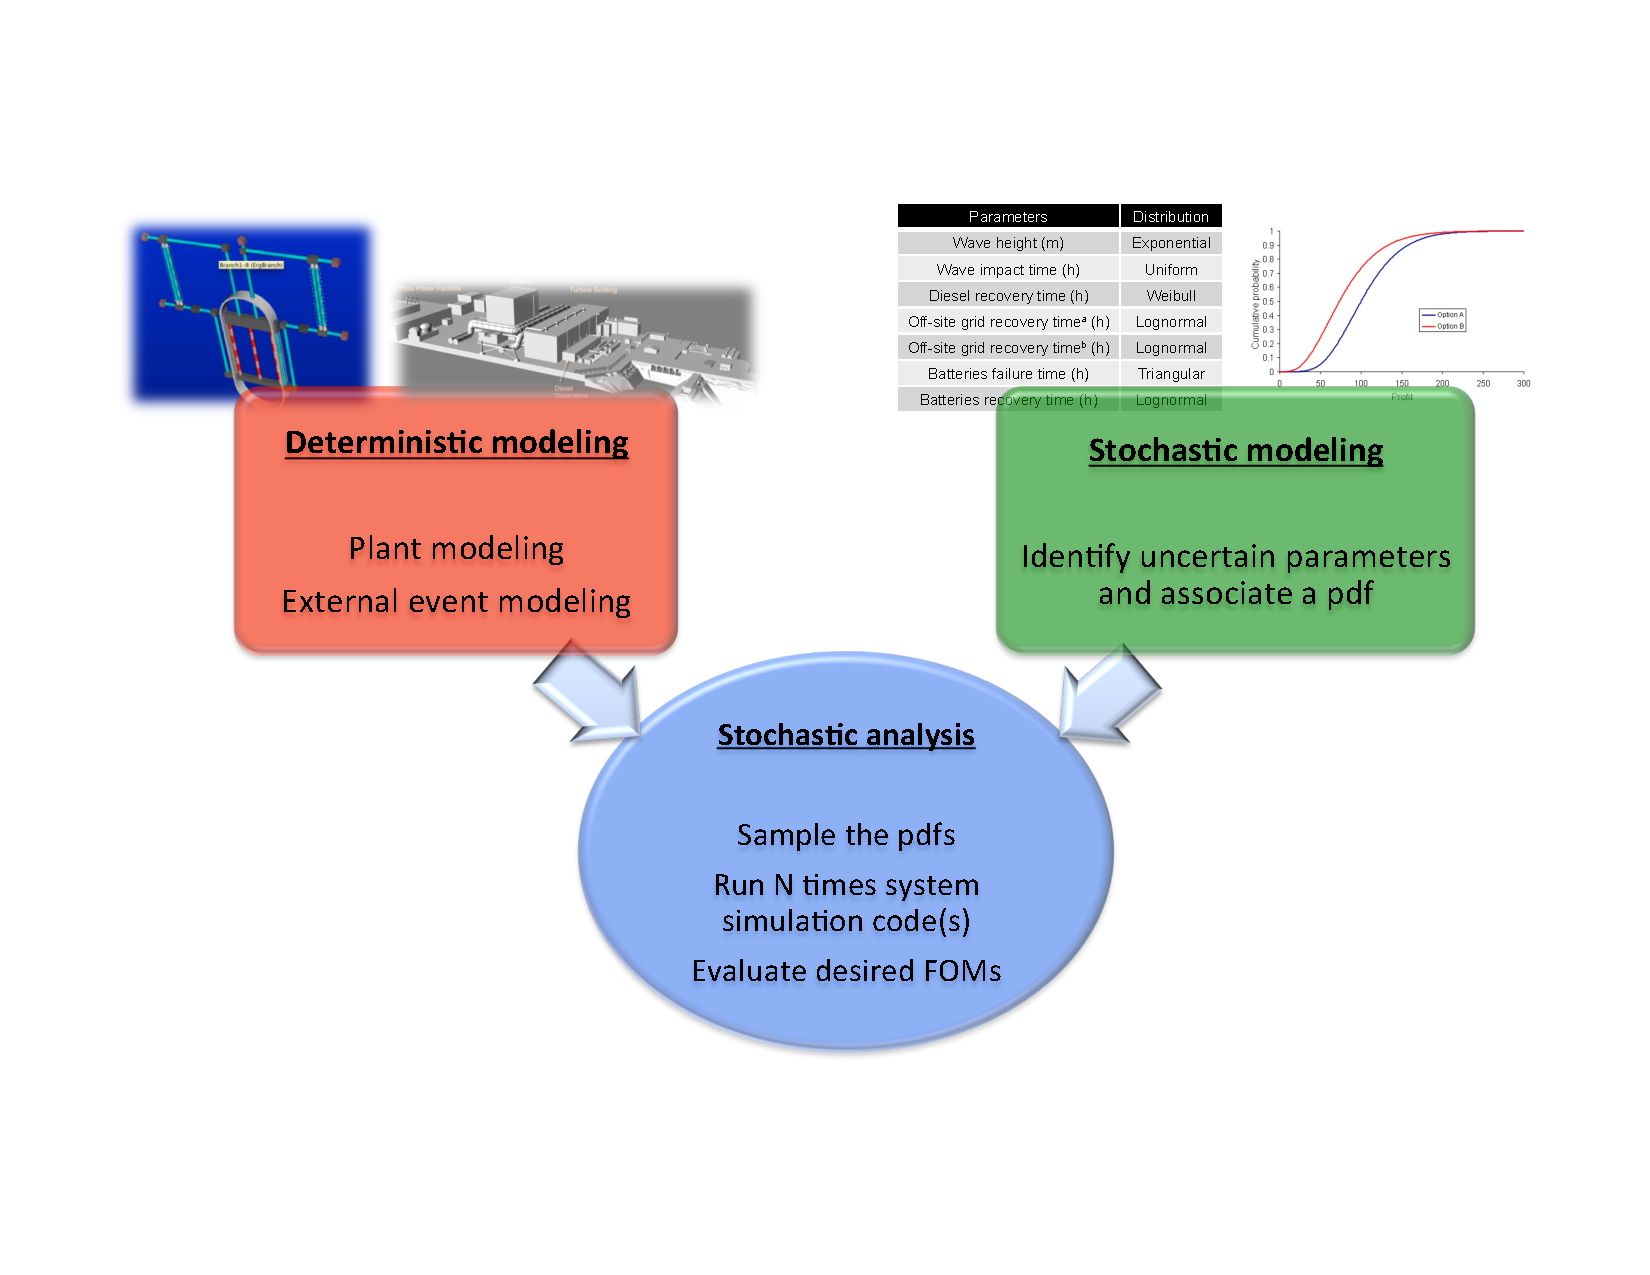
\includegraphics[scale=0.4]{RISMCoverview.pdf}}
    \caption{Overview of the RISMC approach}
    \label{fig:RISMCoverview}
\end{figure}

Note that deterministic modeling of the plant or external events can be performed by employing specific 
simulator codes but also surrogate models~\cite{ROM}, known as reduced order models (ROM). ROMs would 
be employed 
in order to decrease the high computational costs of employed codes. In addition, multi-fidelity codes 
can be employed to model the same system; the idea is to switch from low-fidelity to high-fidelity code 
when higher accuracy is needed (e.g., use low-fidelity codes for steady-state conditions and high-fidelity 
code for transient conditions)

In the stochastic modeling we include all stochastic parameters that are of interest in the PRA analysis 
such as uncertain parameters and stochastic failure of system/components.
As mentioned earlier, the RISMC approach heavily relies on multi-physics system simulator codes 
(e.g., RELAP5-3D~\cite{relap5}) coupled with stochastic analysis tools (e.g., RAVEN~\cite{raven}).  
From a PRA point of view, this type of simulation can be described by using two sets of variables:
\begin{itemize}
  \item $\boldsymbol c = \boldsymbol c(t)$ represents the status of components and systems of the simulator 
        (e.g., status of emergency core cooling system, AC system)
  \item $\boldsymbol \theta = \boldsymbol \theta (t)$ represents the temporal evolution of a simulated 
        accident scenario, i.e., $\boldsymbol \theta (t)$ represents a single simulation run. 
        Each element of $\boldsymbol \theta$ can be for example the values of temperature or pressure in 
        a specific node of the simulator nodalization.
\end{itemize}

From a mathematical point of view, a single simulator run can be represented as a single trajectory in the 
phase space. The evolution of such a trajectory in the phase space can be described as follows:
\begin{equation}
  \begin{cases}
    \dfrac{\partial \boldsymbol \theta }{\partial t}  = \boldsymbol \Xi (\boldsymbol \theta , \boldsymbol c, \boldsymbol s , t)   \\ \\ 
    \dfrac{\partial \boldsymbol c }{\partial t}  = \boldsymbol \Gamma (\boldsymbol \theta , \boldsymbol c, \boldsymbol s , t) 
  \end{cases}    
  \label{eq:trajectory}
\end{equation}
where:
\begin{itemize}
  \item $\boldsymbol \Xi$ is the actual simulator code that describes how θ evolves in time
  \item $\boldsymbol \Gamma$ is the operator which describes how c evolves in time , i.e., the status 
        of components and systems at each time step
  \item $\boldsymbol C$ is the set of stochastic parameters.
\end{itemize}

Starting from the system located in an initial state, $\boldsymbol \theta (t=0) = \boldsymbol \theta(0)$, 
and the set of stochastic parameters (which are generally generated through a stochastic sampling process), 
the simulator determine at each 
time step the temporal evolution of $\boldsymbol \theta (t)$. At the same time, the system control logic  
determines the status of the system and components $\boldsymbol c(t)$.
 
By using the RISMC approach, the PRA analysis is performed by~\cite{}:
\begin{enumerate}
  \item Associating a probabilistic distribution function (pdf) to the set of parameters 
        $\boldsymbol s$ (e.g., timing of events)
  \item Performing stochastic sampling of the pdfs defined in Step 1
  \item Performing a simulation run given $\boldsymbol s$ sampled in Step 2, i.e., solve the 
        system of equations~\ref{??}
  \item Repeating Steps 2 and 3 $M$ times and evaluating user defined stochastic parameters such 
        as core damage (CD) probability ($P_{CD}$).
\end{enumerate}

\section{RISMC Approach and Classical PRA}
\label{sec:analogy}

In order to better understand the results obtained in Section~\ref{sec:test} it is worth to illustrate 
a link between classical PRA and RISMC approach.
Let's consider a system that is composed by two components (i.e, A and B) in a series configuration where
each component has a failure probability (i.e., $p_A$ and $p_B$ respectively) as shown in Fig.~ref{}.

In a classical PRA framework such system can be modeled using a FT method that is composed by two basic events:
A failed and B failed.
System failure would be represented by a single ``AND'' gate that combine the two basic events as shown in 
Fig.~ref{}.

\begin{figure}
  \centering
  \begin{subfigure}{.5\textwidth}
    \centering
    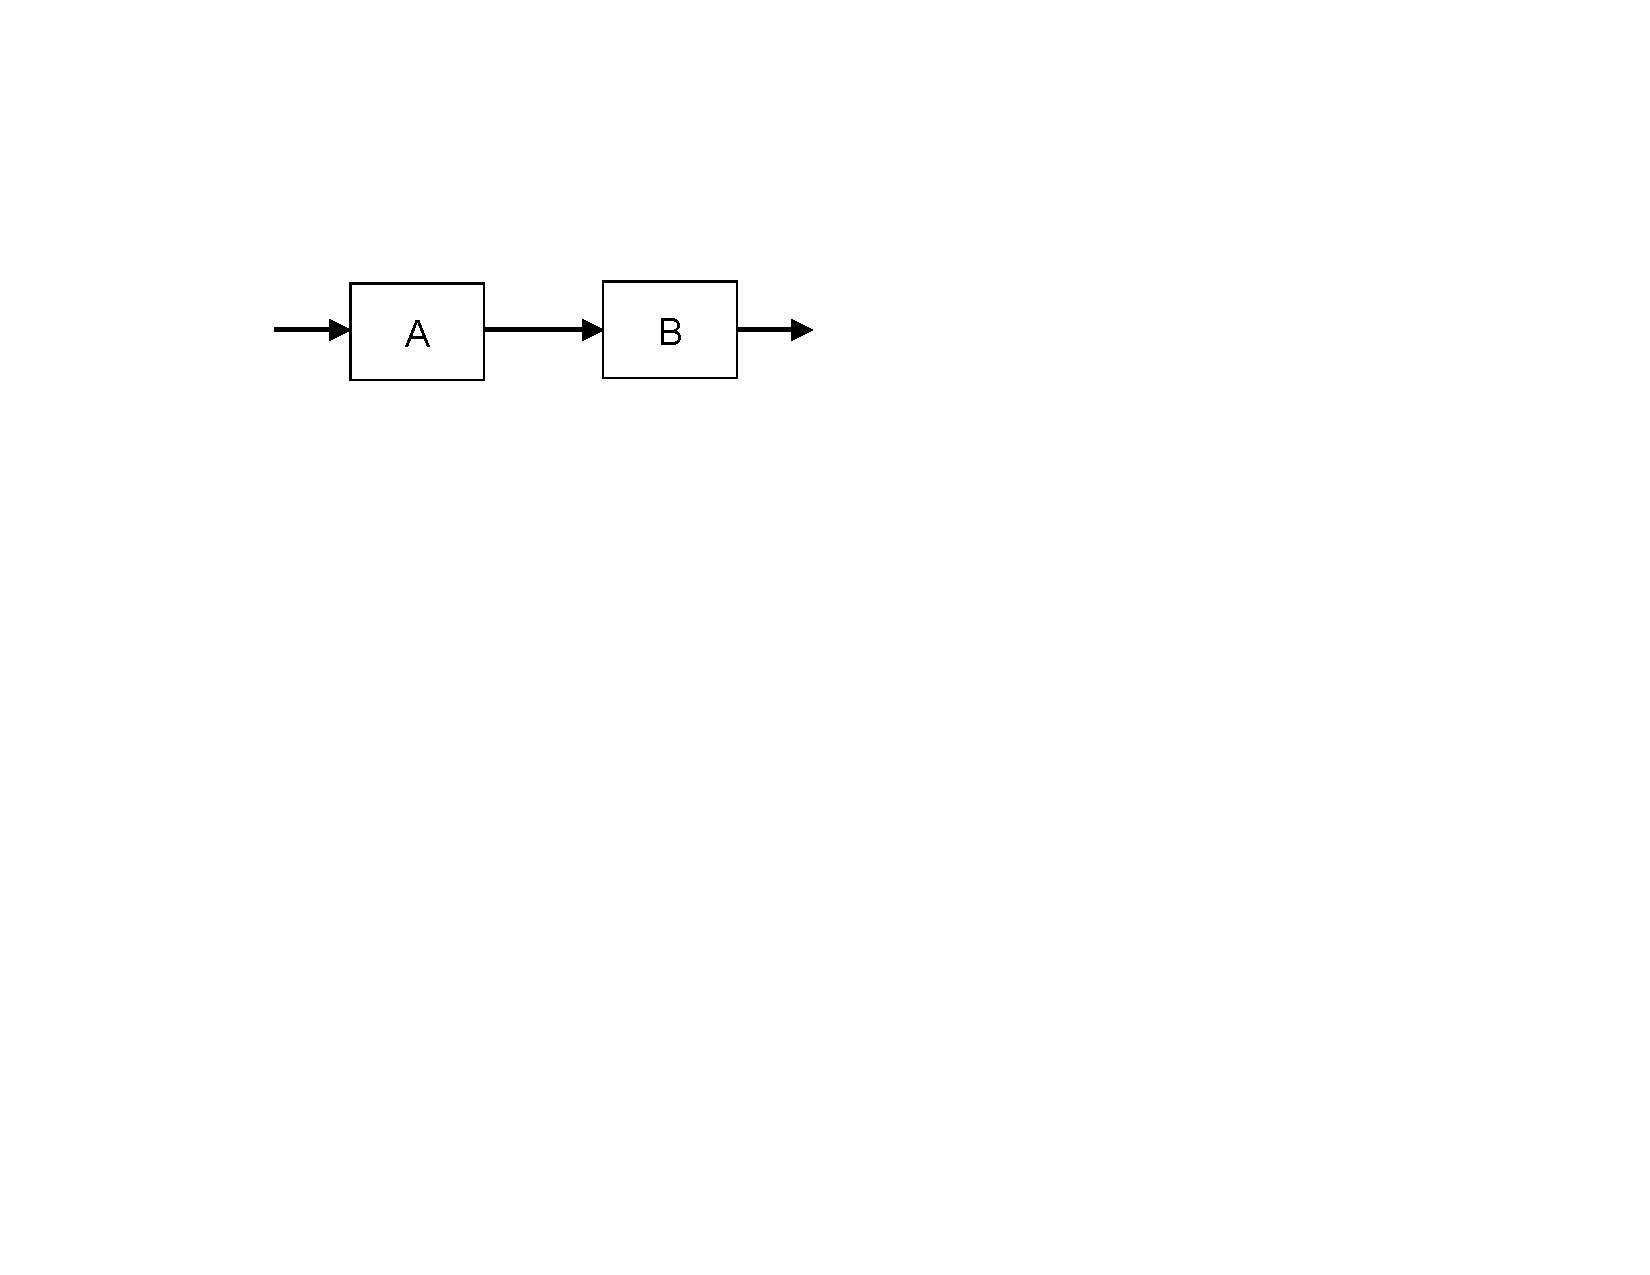
\includegraphics[scale=0.6]{ABsystem.pdf}
    \label{fig:sub1}
  \end{subfigure}%
  \begin{subfigure}{.5\textwidth}
    \centering
    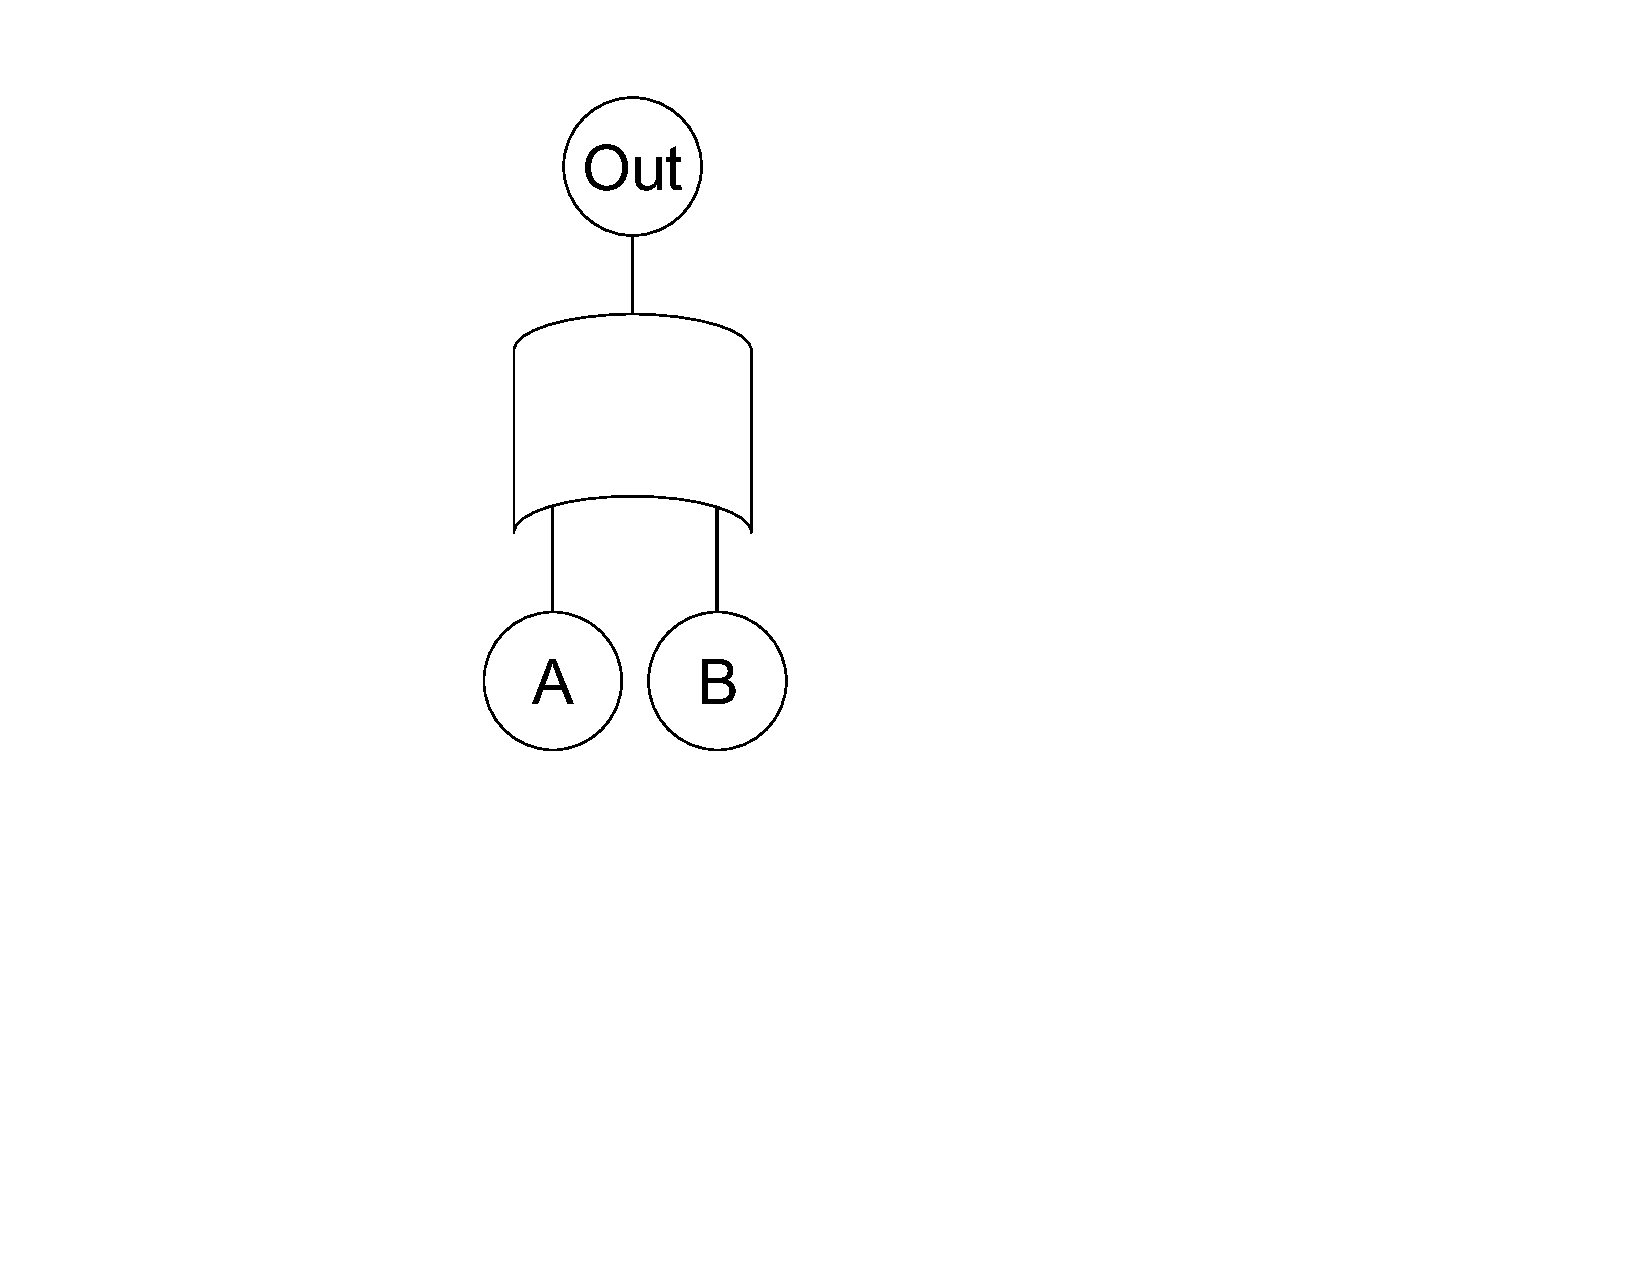
\includegraphics[scale=0.3]{andGate.pdf}
    \label{fig:sub2}
  \end{subfigure}
  \caption{Components A and B in a series configuration (left) and associated Fault-Tree (right).}
  \label{fig:chebyshev}
\end{figure}

\begin{figure}
    \centering
    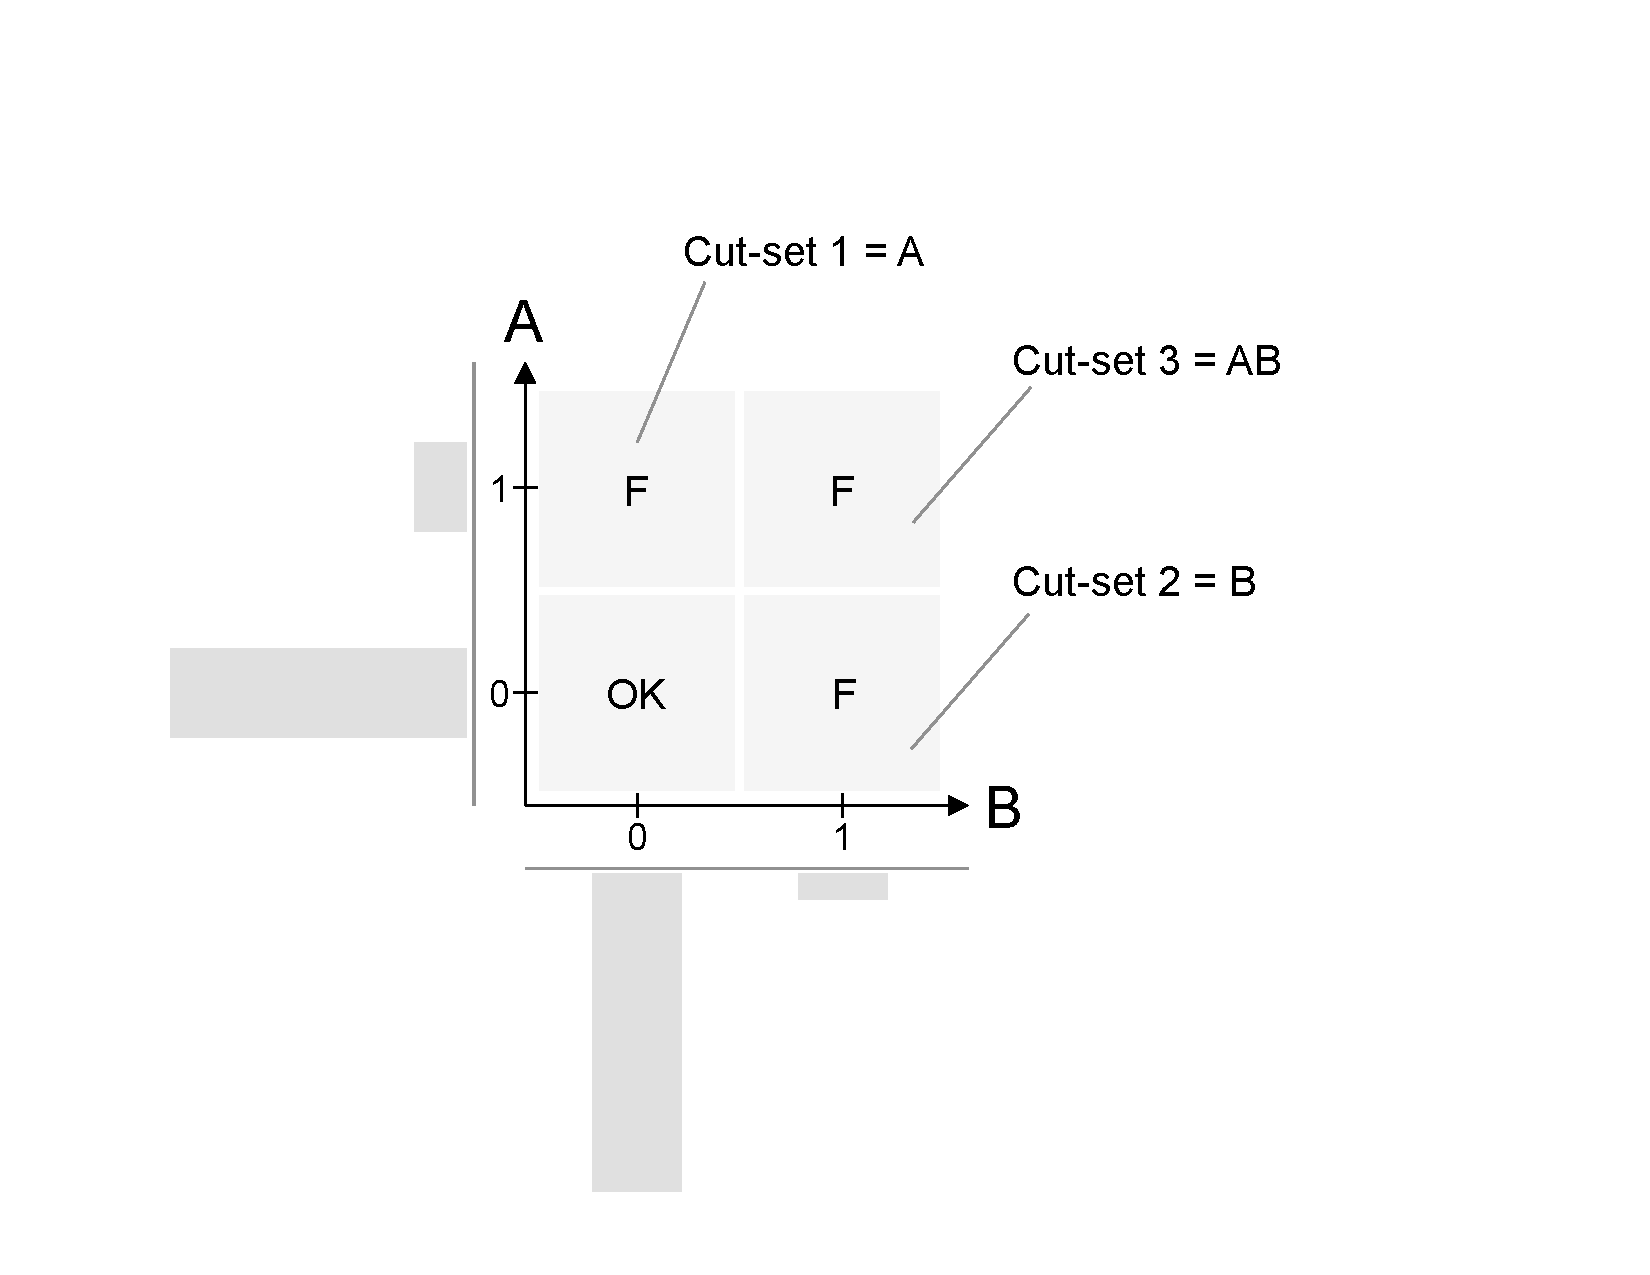
\includegraphics[scale=0.4]{2D.pdf}
    \caption{}
    \label{fig:2Danalogy}
\end{figure} 




\section{RAVEN}
\label{sec:raven}
 
The Risk Analysis and Virtual ENviroment 
(RAVEN\footnote{Official website: \url{https://raven.inl.gov},\\ 
GITHUB repository: \url{https://github.com/idaholab/raven}})
~\cite{RAVEN_PSAM_2014,alfonsiEsrel2014} 
is a flexible and multi-purpose uncertainty quantification, regression analysis, probabilistic
risk assessment, data analysis and model optimization framework. Depending on the tasks to be 
accomplished and on the probabilistic characterization of the problem, RAVEN perturbs 
(e.g., Monte-Carlo, latin hypercube, reliability surface search) the response of the system 
under consideration by altering its own parameters. The system is modeled by third party software 
(e.g., RELAP5-3D~\cite{relap5}, MELCOR~\cite{Melcor}) and accessible to RAVEN either directly 
(software coupling) or indirectly (via input/output files). 
The data generated by the sampling process is analyzed using 
classical statistical and more advanced data mining approaches. RAVEN also manages the parallel dispatching 
(i.e. both on desktop/workstation and large High Performance Computing machines) of the software 
representing the physical model. RAVEN heavily relies on artificial intelligence algorithms to construct 
surrogate models of complex physical systems in order to perform uncertainty quantification, reliability 
analysis (limit state surface) and parametric studies.

By statistical analysis we include:
\begin{itemize}
  \item Sampling of codes, either stochastic, e.g., Monte-Carlo~\cite{DynamicReliabilityMonteCarlo} 
        and Latin Hypercube Sampling (LHS)~\cite{LHShelton}, deterministic (e.g., grid and
        Dynamic Event Tree (DET)~\cite{AMENDOLAdylam,cojazziDylam}) or 
        adaptive~\cite{ANS_S_2014_raven_LS,mandelliSVMANS}
  \item Generation of ROMs~\cite{ROM_Khalik}, also known as Surrogate models
  \item Post-processing of the sampled data and generation of statistical parameters (e.g., mean, 
        variance, covariance matrix).
\end{itemize}

Figure~\ref{fig:ravenScheme} shows a general overview of the elements that comprise the RAVEN 
statistical framework:

\begin{itemize}
  \item Model: it represents the pipeline between input and output space. It comprises both codes 
        (e.g., RELAP5-3D~\cite{relap5}) and also ROMs 
  \item Sampler: it is the driver for any specific sampling strategy, e.g., Monte-Carlo, LHS, 
        DET~\cite{ANS2014_adaptDET,PSA2013_Raven})
  \item Database: the data storing entity
  \item Post-processing module: the module that performs statistical analyses and visualizes results.
\end{itemize}

\begin{figure}
    \centering
    \centerline{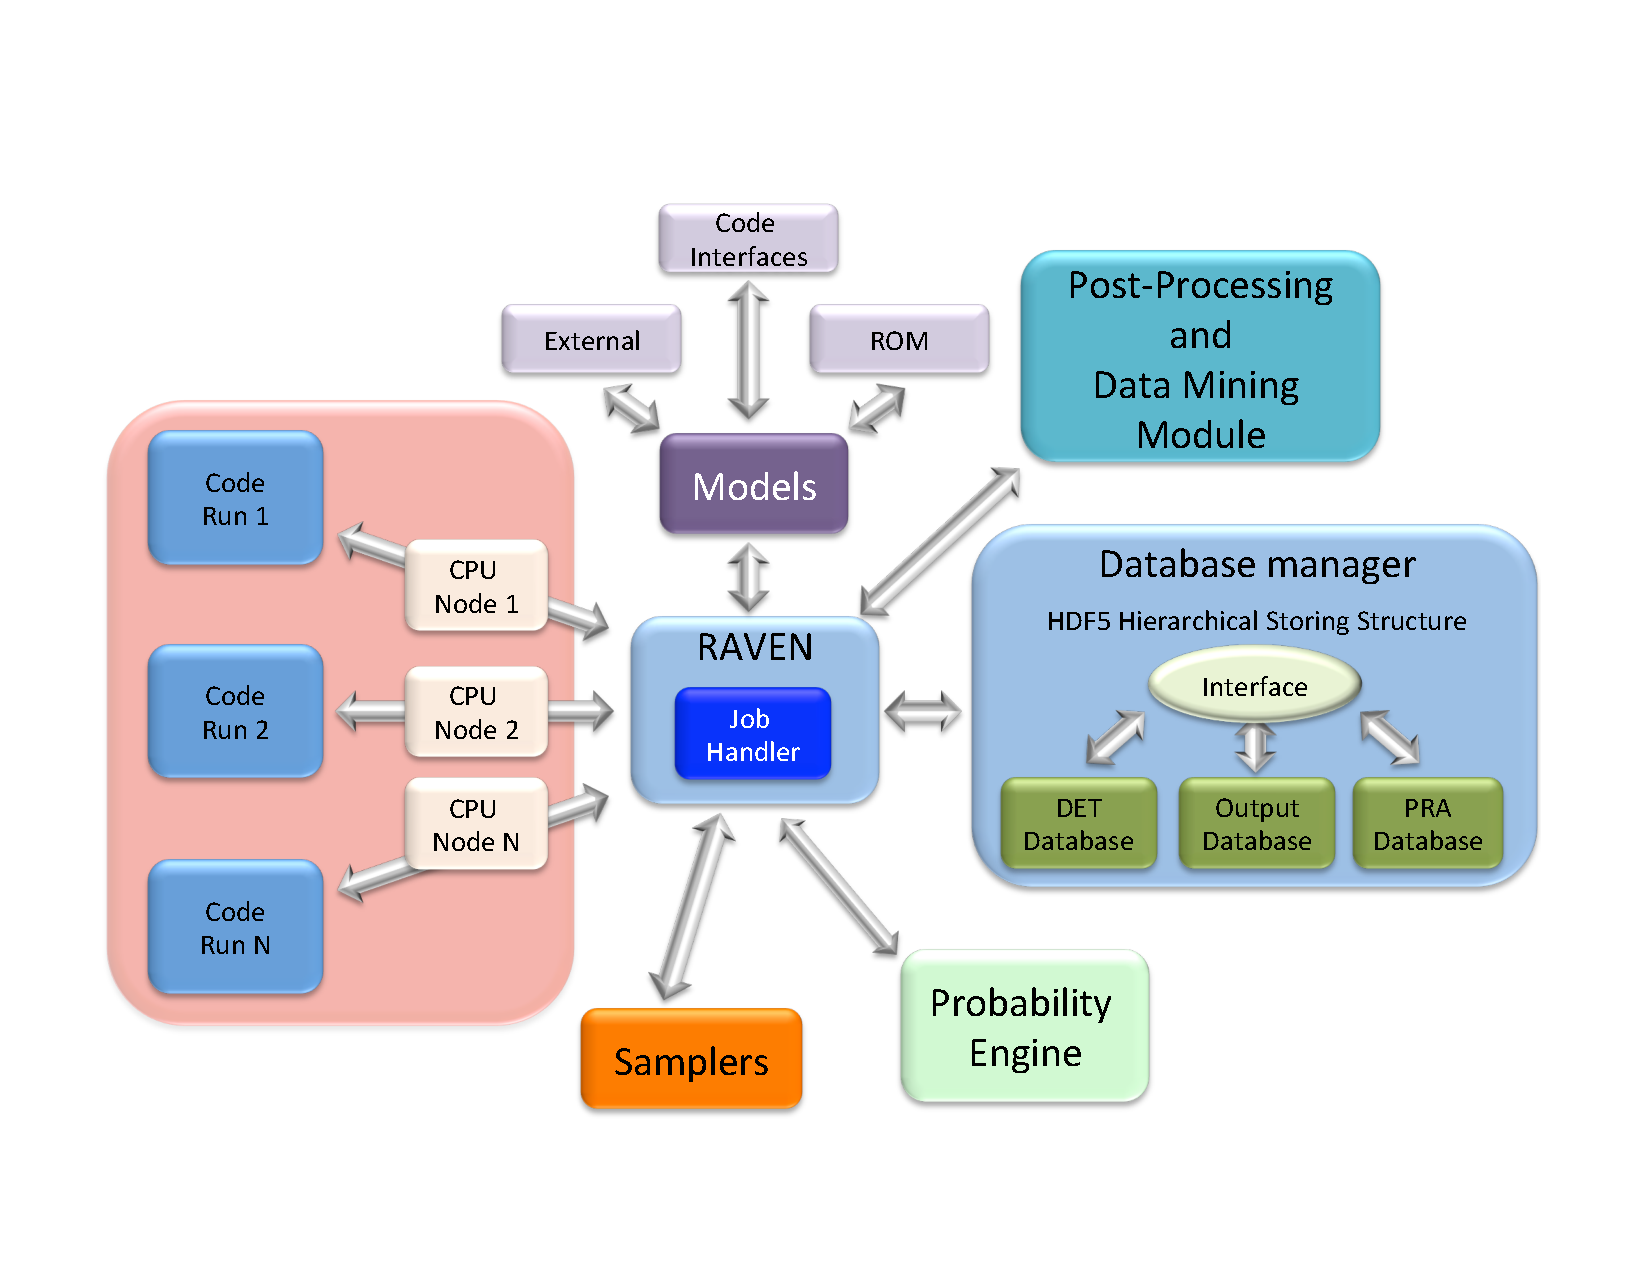
\includegraphics[scale=0.4]{raven.pdf}} 
    \caption{Overview of RAVEN statistical framework components}
    \label{fig:ravenScheme}
\end{figure}


\section{Classical Rims In A Dynamic Pra Context}
\label{sec:classicalRIMs_RISMC}

In a Dynamic PRA environment, $R_0$ is obtained (e.g., through Monte-Carlo sampling) by:
\begin{enumerate}
  \item Running $N$ simulation (e.g., RELAP5 runs)
  \item Counting the number $N_{CD}$ of simulations that lead to core damage (CD) condition
  \item Calculating $R_0= \frac{N_CD}{N}$
\end{enumerate}
Note that while basic events in classical PRA are mainly Boolean, in a Dynamic PRA environment the 
sample parameters can be, not only Boolean, but more often continuous. As an example, let consider
two basic events:
\begin{itemize}
  \item Emergency Diesel Generator (EDG) failure to start, and, 
  \item EDG failure to run
\end{itemize}

In classical PRA analyses, a probability value is associated to each basic event. On the other side, 
in a Dynamic PRA framework, a Bernoulli distribution could be associated to the first basic event and 
a continuous distribution (e.g., exponential distribution) could be associated to the second basic event. 
At this point a challenge arises: the determination of $R_i^-$ and $R_i^+$ for each sampled parameter; 
two possible approaches can be followed :
\begin{enumerate}
  \item Perform a Dynamic PRA for $R_0$ and each $R_i^-$ and $R_i^+$
  \item Determine an approximated value of $R_i^-$ and $R_i^+$ from the simulation runs generated to calculate $R_0$
\end{enumerate}
Regarding Approach 1, given the computational costs of each Dynamic PRA, it is unfeasible to determine 
$R_i^-$ and $R_i^+$ for each sampled parameter. In fact, if we consider $M$ sample
parameters (i.e., $S$ basic events), then the risk importance analysis would require $2S+1$ Dynamic PRA analyses.

Regarding Approach 2, a method (implemented in RAVEN as an internal post-processor) was developed and it is 
here presented. This method requires an input from the user:
\begin{itemize}
  \item Range, $I_i^-$, of the variable $s_i$ that can be associated to ``basic event with component perfectly reliable''
  \item Range, $I_i^+$, of the variable $s_i$ that can be associated to ``basic event in a failed status''
\end{itemize}
Given this kind of information, it is possible to calculate $R_i^+$ and $R_i^-$ as follows:
\begin{align} 
  R_0   &= \frac{N_{CD}}{N}  \\
  R_i^+ &= \frac{N_{CD, s_i \in I_i^+}}{N}   \\
  R_i^- &= \frac{N_{CD, s_i \in I_i^-}}{N} 
\end{align}
where:
\begin{itemize}
  \item $N_{CD, s_i \in I_i^+}$ as the number of simulations leading to core damage and with parameter $s_i \in I_i^+$
  \item $N_{CD, s_i \in I_i^-}$ as the number of simulations leading to core damage and with parameter $s_i \in I_i^-$
\end{itemize}

Note that this approach has an issue related to the choices of $I_i^+$ and $I_i^-$. 
Depending on their values, $R_i^+$ and $R_i^-$ might change accordingly. In addition, the statistical error 
associated to the estimates of $R_i^+$ and $R_i^-$ also changes. 
An example is shown in Figure 1 for both cases (discrete and continuous) of a basic event $x_i$ represented 
as a stochastic variable which is sampled (e.g., through a Monte-Carlo process) for each simulation run.
Lets consider the continuous case and assume $s_i$ correspond to the basic event ``EDG failure to run''. 
The user might impose the following in order to determine $R_i^+$ and $R_i^-$:
\begin{itemize}
  \item $I_i^-=[T_i^-,\infty]$ where $T_i^-$ may be set equal to the simulation mission time (e.g., 24 hours). 
        This implies that a sampled value for EDG failure to run greater than 24 hours implies that the 
        EDG actually does not fail to run (reliability equal to 1.0)
  \item $I_i^+=[0,T_i^+ ]$ where $T_i^-$ may be set to an arbitrary small value (e.g., 5 min). This implies that 
        a sampled value for EDG failure to run smaller than 5 min implies a reliability equal to 0.0
\end{itemize}

Note that while the definition of $I_i^-$ is perfectly reasonable, one would argue that a smaller interval 
should be chosen for $I_i^+$ (e.g., 30 seconds or less). 
Recall that ideally, a value of $s_i=0.0$ should be theoretically chosen (and not an interval); however, 
given the nature of the distribution this is not allowed. Given the nature of the problem, we are bound 
to choose an interval $I_i^+$:
\begin{itemize}
  \item A small interval in the neighbor of $s_i=0.0$ would lead to a value of $R_i^+$ close to the theoretical 
        one. 
        However, the number of actual sampled values falling in $I_i^+$ would be very small, i.e., large stochastic 
        error.
  \item A large interval in the neighbor of $s_i=0.0$ would lead to a value of $R_i^+$ far from the theoretical one. 
        However, the number of actual sampled values falling in $I_i^+$ would be very high,
        i.e., small stochastic error.
\end{itemize}

A solution to the large statistical error associated to a very small interval $I_i^+$ can be solved by 
employing different sampling algorithms other than the classical Monte-Carlo one. 
As an example, a better resolution of the final value for $R_i^+$ can be achieved by sampling uniformly 
the range of variability of $x_i$ and associate an importance weight to each sample. At this point
the counting variable $N_{CD}$ is weighted by the weight of each sample. By sampling uniformly the range of 
variability of $x_i$, the number of samples in the interval $I_i^+$ would be significantly higher.

\begin{figure}
    \centering
    \centerline{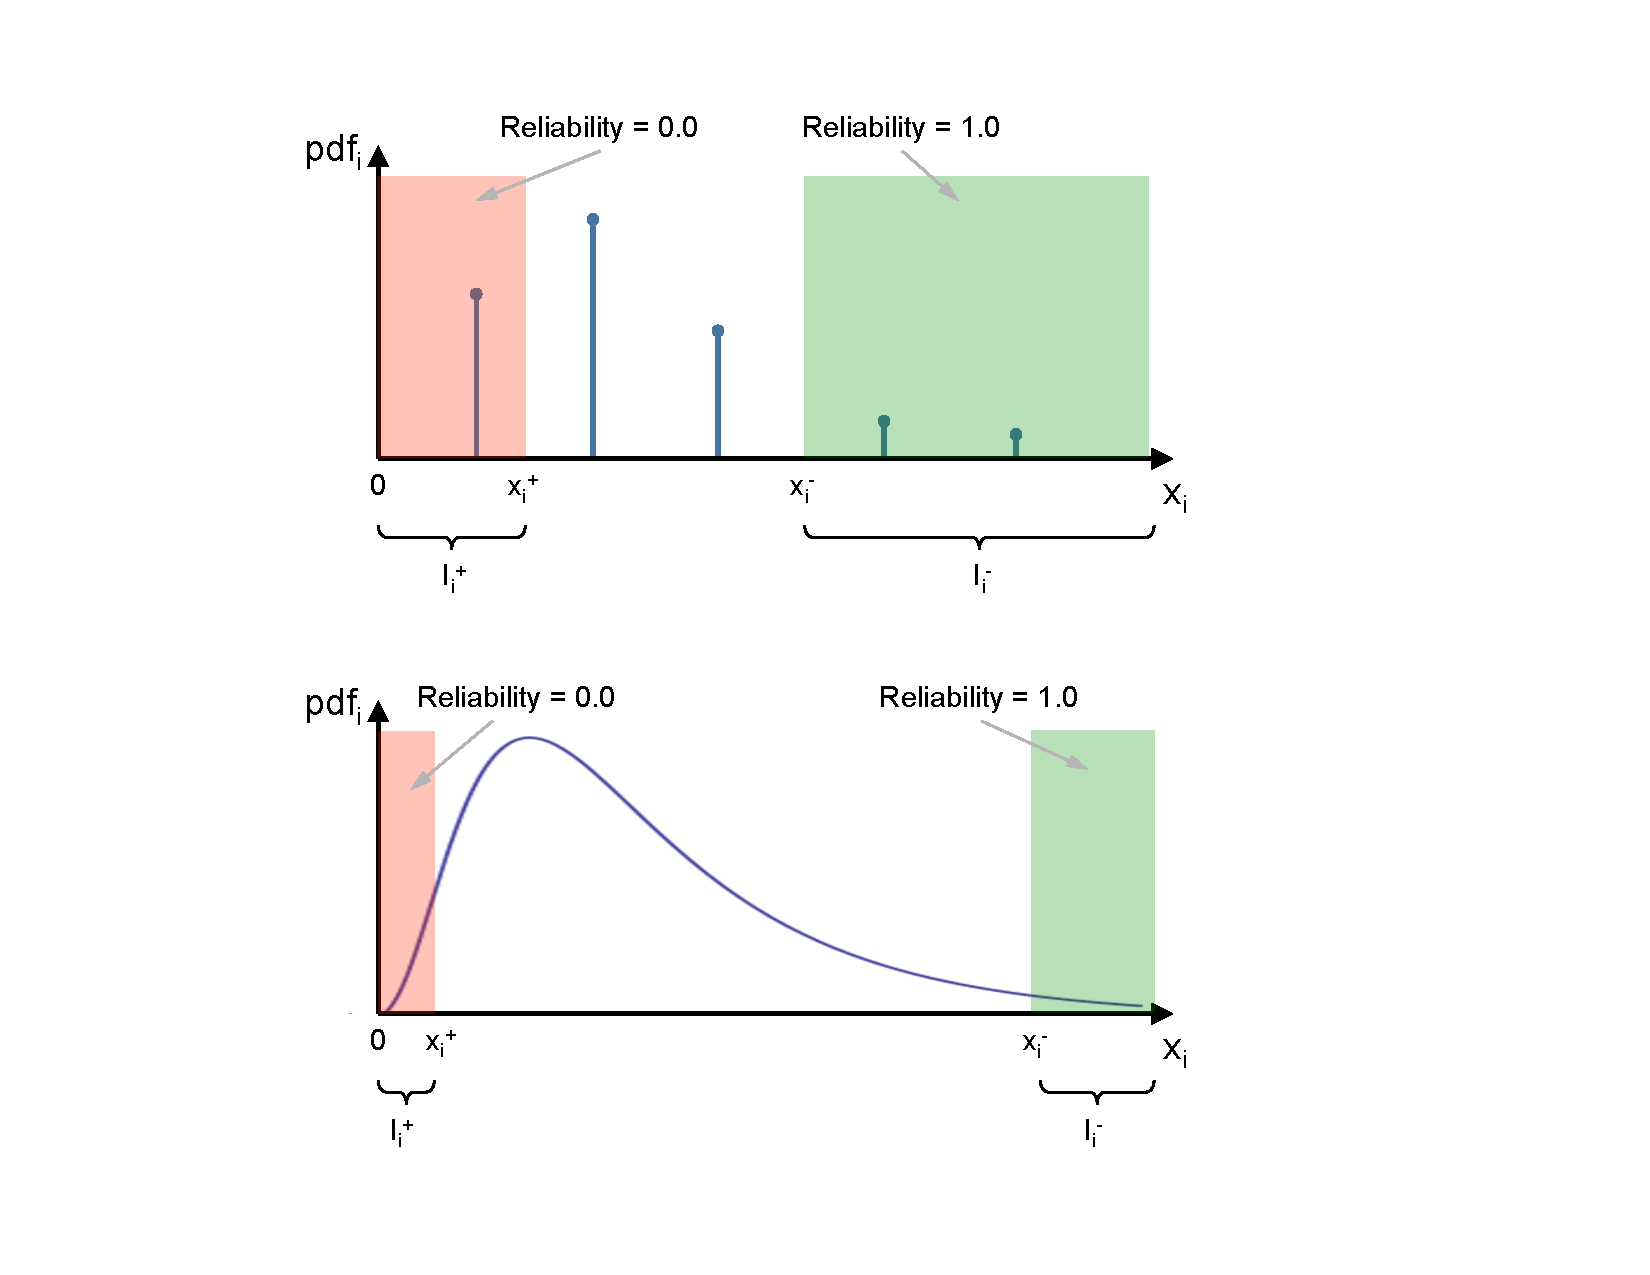
\includegraphics[scale=0.5]{intervals.pdf}} 
    \caption{Treatment of discrete (top) and continuous (bottom) stochastic variables for reliability purposes.}
    \label{fig:intervals}
\end{figure}

\section{Test Examples}
\label{sec:test}

In this section we present few examples that will help the reader to understand 
how this method can be applied to fairly common cases.

\subsection{Example 1: series/parallel configuration}
\label{sec:example1}

The first example is shown in Fig.~\ref{}: it consists of 3 components arranged 
in a series/parallel 
configuration. In this case the following probabilities of failures (on-demand) 
are provided:
\begin{itemize}
  \item $p_A = 1.0 10^{-2}$
  \item $p_B = 5.0 10^{-2}$
  \item $p_C = 1.0 10^{-1}$
\end{itemize}
  
From a dynamic PRA point of view the analysis of this system is performed as follows:
\begin{itemize}
  \item Define 3 stochastic parameters (i.e., $S=3$):
    \begin{itemize}
      \item $s_1$: status of component A
      \item $s_2$: status of component B
      \item $s_3$: status of component C
    \end{itemize}
  \item Assign a distribution to each stochastic parameter; in this case a Bernoulli 
        distribution  
  \item Define $I_i^+$ and $I_i^-$ for each distribution: in this case we have chosen 
        $I_i^-=[0.0,0.1]$ and $I_i^+=[1.0,1.1]$ 
  \item Generate $N$ samples, for example by Monte-Carlo sampling 
  \item Determine $R_0$, $R_i^-$ and $R_i^+$ for each component 
  \item Determine the desired RIMs for each component
\end{itemize}

Note that a Monte-Carlo sampling is not the best sampling strategy in terms of computational 
costs. This is even more relevant if the value of $p_A$, $p_B$ or $p_C$ were several order of 
magnitude lower. 

A more effective sampling strategy would be the Grid sampling: the stochastic variables 
are sampled over a fixed Cartesian grid and a probability weight is associated to each sample. 
In this case, each stochastic variable $s_i$ is sampled over two values, 0.0 and 1.0, and the 
probability weights $w_i^0$ and $w_i^1$ values associated to each sample coordinate are:
\begin{itemize}
  \item $s_i=0.0$: $w_i^0=prob(s_i \in [-\infty,0.5])$
  \item $s_i=1.0$: $w_i^1=prob(s_i \in [0.5,+\infty])$
\end{itemize}
Following this grid sampling strategy, only $2^N=8$ are needed.
Below, the FV importance for all three components obtained by RAVEN (using a Grid sampling 
strategy) are shown compared with the analytical ones.

\begin{table}
  \caption{Results obtained for Example I.} 
  \centering 
  \begin{tabular}{c | c | c } 
    \hline 
     & Analytical & RAVEN \\ 
    \hline 
    $FV_A$ & 0.6656 & 0.6656   \\
    $FV_B$ & 0.3311 & 0.3311   \\
    $FV_C$ & 0.3311 & 0.3311   \\
    \hline 
  \end{tabular}
  \label{tab:example1} 
\end{table}

\subsection{Example 2: Time-dependent system}
\label{sec:example2}

The second example is similar to Example I but with different reliability data: 
a failure rate is provided for each component (mission time: 24 hours): 
\begin{itemize}
  \item $\lambda_A = 1.0 10^{-3} hr^{-1}$
  \item $\lambda_B = 5.0 10^{-3} hr^{-1}$
  \item $\lambda_C = 1.0 10^{-2} hr^{-1}$
\end{itemize}
Thus it is assumed that failure probability of each component is exponentially 
distributed: sampled value $s_i$ from its own distribution is failure time of each 
component ($t_A$, $t_B$ and $t_C$).
In this case, $I_i^+$ and $I_i^-$ can be defined as follows:
\begin{itemize}
  \item $I_i^-=[24.0,+\infty]$: component is considered perfectly reliable if the failure 
        time is greater than the mission time
  \item $I_i^+=[0.0,1.0]$: component is considered unreliable if the failure time 
        occurs within the first hour
\end{itemize}

As shown for Example I, a Grid sampling strategy has been employed. Table~\ref{} shows the 
FV importance for all three components obtained by RAVEN (using a Grid sampling strategy) 
compared with the analytical ones.

\begin{table}
  \caption{Results obtained for Example II.} 
  \centering 
  \begin{tabular}{c | c | c } 
    \hline 
     & Analytical & RAVEN \\ 
    \hline 
    $FV_A$ & 0.48957 & 0.48957  \\
    $FV_B$ & 0.4983  & 0.4983   \\
    $FV_C$ & 0.4983  & 0.4983   \\
    \hline 
  \end{tabular}
  \label{tab:example2} 
\end{table}

\subsection{Example 3: stand-by configuration}
\label{sec:example3}

The third example considers a simplified ECCS model (see Fig.~\ref{}) for a Pressurized 
Water Reactor (PWR). It consists of the following components and for a subset of them a 
value of mean time to failure (MTTF) is provided:
\begin{itemize}
  \item Motor-operate valve M (MTTF = 24 h)
  \item Two redundant pumps, pump1 and pump2 (MTTF = 12 h)
  \item Heat exchanger HX (reliability = 1.0)
\end{itemize}

Pump1 is normally used while pump2 is on standby. If Pump1 fails then pump2 provide water flow. 
Pump2 cannot fail while in standby. Switch from pump1 to pump2 is perfectly reliable. 
The cooling is such that it takes 2 hours to reach vessel failure condition if the M-pump1-pump2 
system has failed. Top event is: overheating of the vessel. Mission time is again equal to 24 hours.

Failure of the system occurs when temperature insider the core reaches a limit temperature. 
Note that the configuration is slightly different from the one presented in the first two 
examples (here a stand-by configuration is introduced) but also the condition of system failure 
is dictated by the dynamic behavior of the PWR.  The system is designed such that a late failure 
of the ECCS may not lead to system failure (i.e., natural circulation is providing enough cooling). 
In other words, the ECCS is vital especially in the hours right after a reactor scram.

\begin{figure}
    \centering
    \centerline{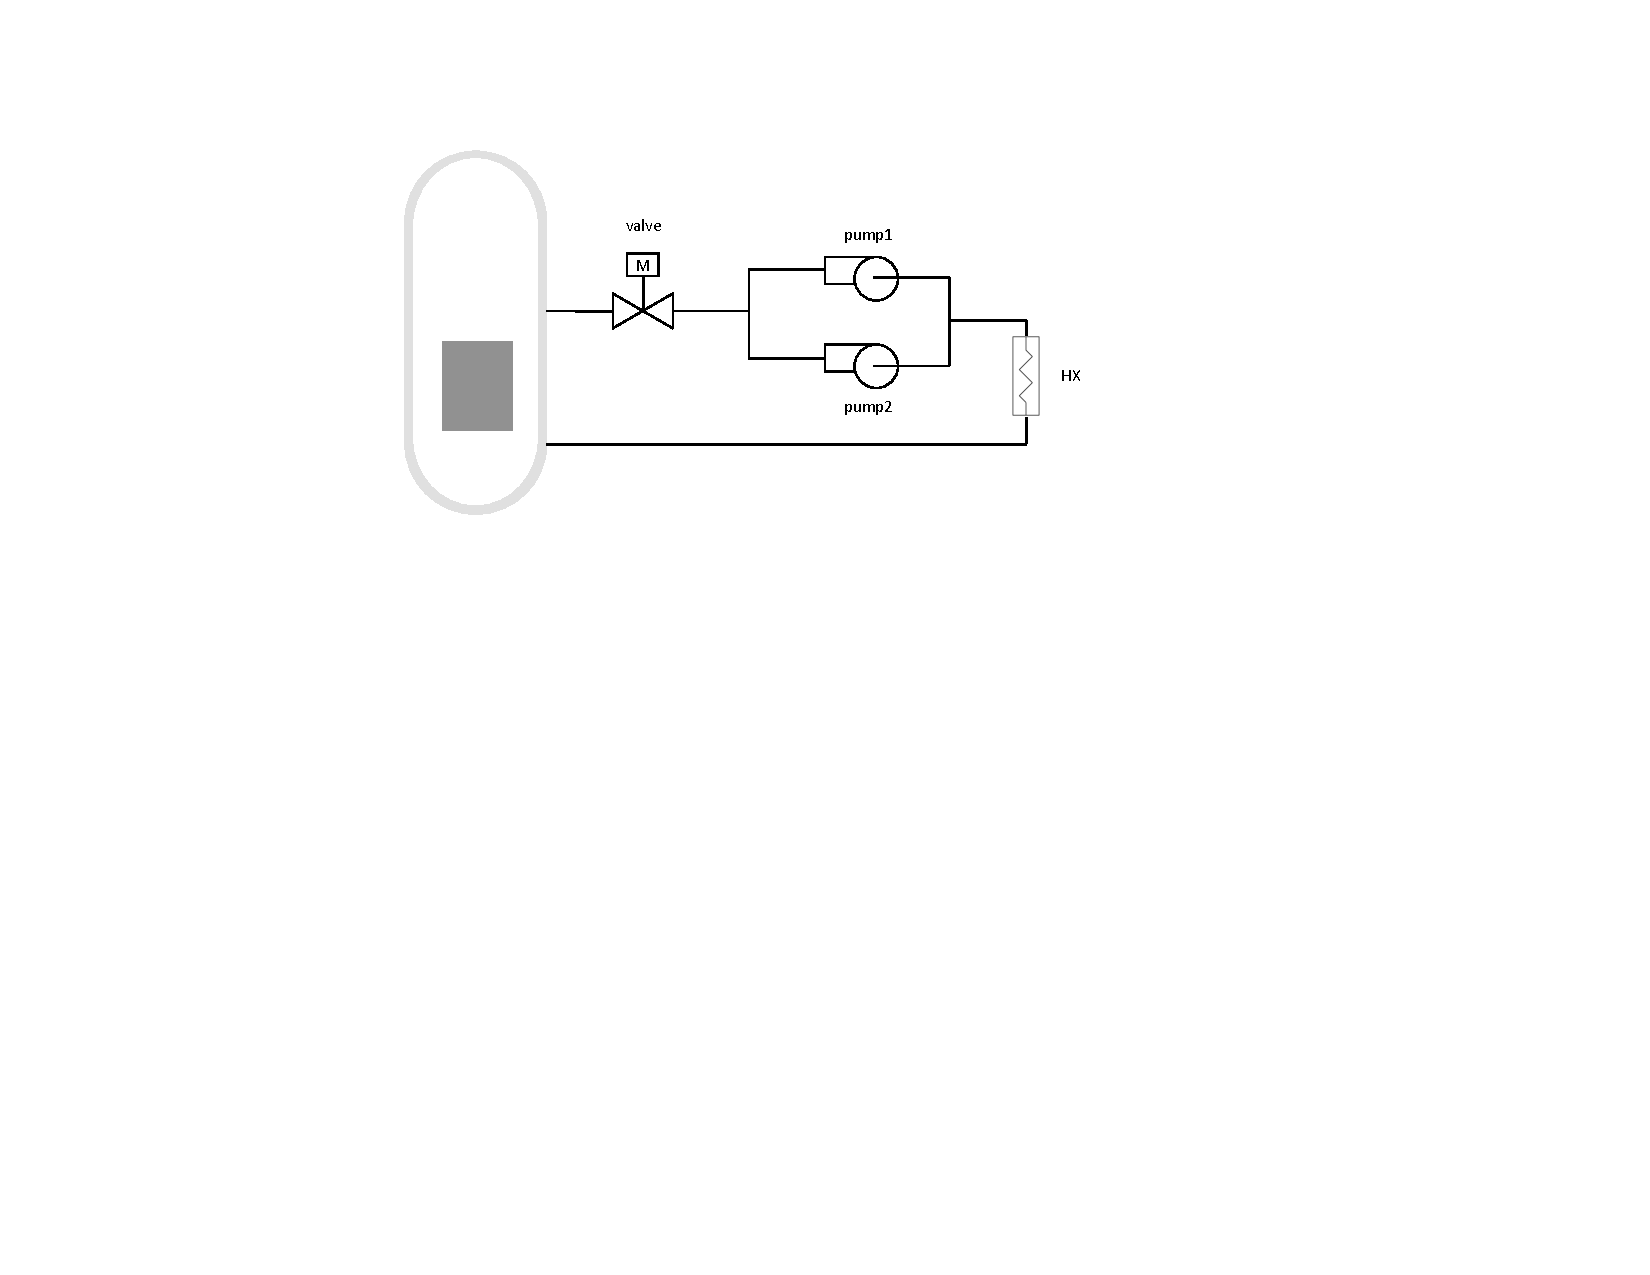
\includegraphics[scale=0.6]{case2.pdf}}
    \caption{System for Example III.}
    \label{fig:example3}
\end{figure}

Note in this case classical PRA methods require few model simplifications in order to correctly 
determine system reliability.
In contrast, a dynamic PRA analysis follows the same steps presented for the first two examples; 
the only difference is represented by the simulator that is actually employed.
Below are shown the FV importance for all three components obtained by RAVEN (using a Monte-Carlo 
sampling strategy) compared with the analytical ones.

\begin{table}
  \caption{Results obtained for Example III.} 
  \centering 
  \begin{tabular}{c | c | c } 
    \hline 
     & Analytical & RAVEN \\ 
    \hline 
    $FV_{pump1}$ &   & 0.25893  \\
    $FV_{pump2}$ &   & 0.25893   \\
    $FV_{valve}$ &   & 0.30331   \\
    \hline 
  \end{tabular}
  \label{tab:example3} 
\end{table}

\subsection{Example 4: $K$ out of $N$ configuration}
\label{sec:example4}

\begin{figure}
    \centering
    \centerline{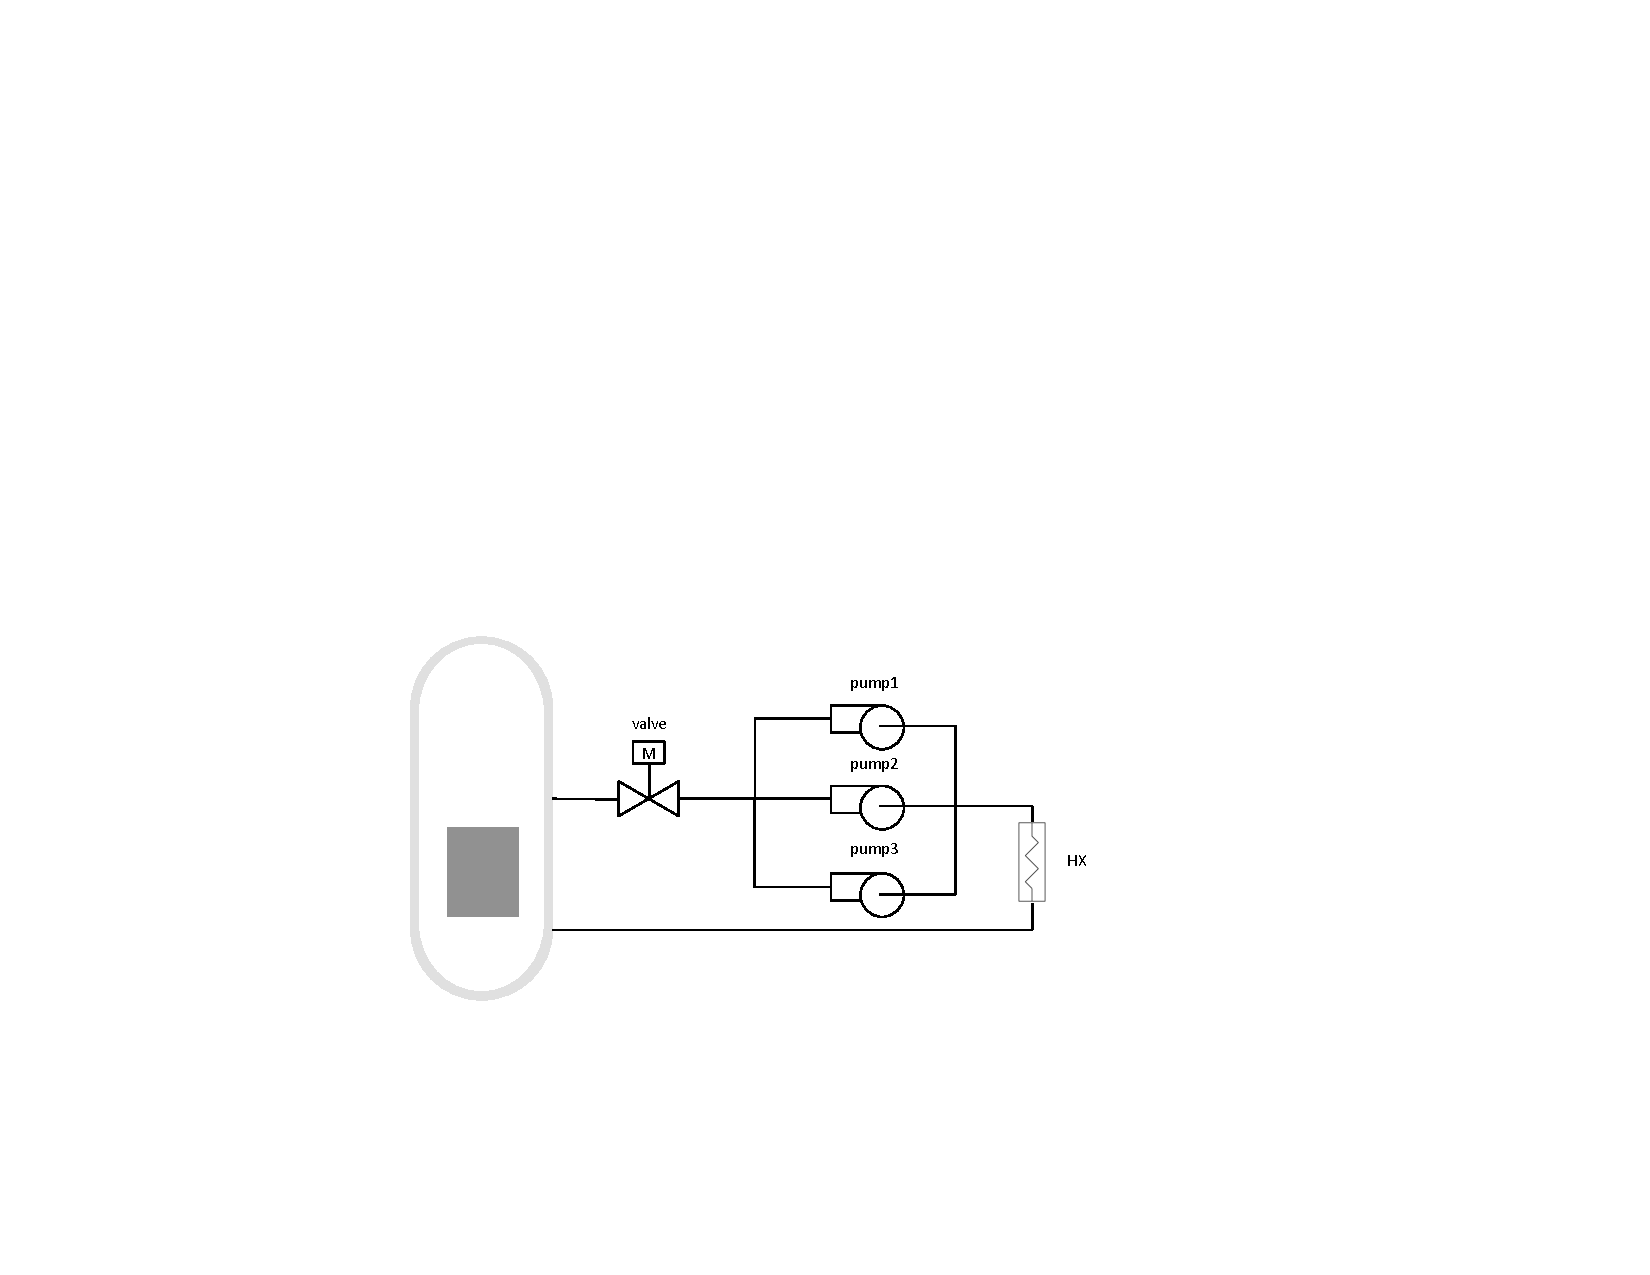
\includegraphics[scale=0.6]{case3.pdf}}
    \caption{System for Example IV.}
    \label{fig:example4}
\end{figure}

\section{Extension To Time-Dependent Data}
\label{sec:timeDepRIMs}

In order to extend the calculation presented above in the time-domain we need 
additional information: the temporal profile of the status of those components 
that might be taken offline due to maintenance or testing.

We will follow this notation:
\begin{itemize}
  \item $\Xi$ represents the system configuration, i.e.,  the status of components 
              and systems of the plant on the time scale $\tau$ of the plant lifetime
  \item $RAW_i(\tau)$, $FV_i(\tau)$, $RRW_i(\tau))$, $B_i(\tau)$ are the RIMs determined 
        for the basic event $i$ calculated on the time scale $\tau$
\end{itemize}

Note that in our application the status of each component can be only binary: 
component operating or component off-line (i.e., either because it is failed or 
under maintenance/testing). Thus component performance degradation is not considered.
The calculation algorithms is as follows given a set of simulated data:
\begin{enumerate}
  \item Divide the temporal profile into $L$ segments where the status of the components,
        i.e. the system configuration $\Xi$, remain constant
  \item For each time segment, i.e., for $l=1,\ldots,L$ 
        \begin{enumerate}
          \item Determine $R_0$ according to the system configuration $\Xi_l$ for segment $l$
            \begin{equation}
              R_0(l) = \frac{N_{CD, \Xi=\Xi_l}}{N_{\Xi=\Xi_l}} 
              \label{eq:}
            \end{equation}
          \item For each component determine $R_i^-$ and $R_i^+$
          \begin{itemize}
            \item If the component is on-line, $R_i^-$ and $R_i^+$ are determined as follows:
              \begin{equation}
                R_i^+(l) = \frac{N_{CD, s_i \in I_i^+, \Xi=\Xi_l}}{N_{\Xi=\Xi_l}} 
                \label{eq:}
              \end{equation}
              
              \begin{equation}
                R_i^-(l) = \frac{N_{CD, s_i \in I_i^-, \Xi=\Xi_l}}{N_{\Xi=\Xi_l}} 
                \label{eq:}
              \end{equation}
            \item If the component is off-line determine $R_i^+(l)$ according to Eq.~\ref{} and 
                 set $R_i^-(l)=R_i^+(l)$
          \end{itemize}
        \end{enumerate}
\end{enumerate}

\section{Test example}
\label{sec:timeDepRIMsExample}

For the scope of this paper we have chosen an elementary example that can help the reader to 
understand the proposed algorithm. This a simple system composed of three components 
(i.e., A, B and C) in a parallel/series configuration. To each component a failure rate is 
provided when the system is called on demand:
\begin{itemize}
  \item $\lambda_A=1.0 \cdot 10^{-3} hr^{-1}$
  \item $\lambda_B=5.0 \cdot 10^{-3} hr^{-1}$
  \item $\lambda_C=1.0 \cdot 10^{-2} hr^{-1}$
\end{itemize}
  
Even though the system can be solved analytically we have chosen a dynamic method to solve it in 
order to show how the proposed methods is implemented. 
By using a Monte-Carlo based Dynamic PRA method, we have generated a database of simulated data 
where each data point is structured as follows:
\begin{itemize}
  \item Input variables: failure time of components A, B and C (i.e., $s_i$) sampled from their 
        own distribution (i.e., exponential with lambda values provided at the beginning of this section)
  \item Output variables: status of the system (either OK or CD)
\end{itemize}

We have selected the temporal profile for two components: A and C as shown in Fig.~\ref{fig:plotStatus_line-line}. 
By following the algorithm presented above it has been possible to determine the temporal profiles of:
\begin{itemize}
  \item system failure probability (see Fig.~\ref{fig:plotR0_line})
  \item RIMs such as FV (see Fig.~\ref{fig:plotFV_line-line-line}) 
\end{itemize}

\begin{figure}
    \centering
    \centerline{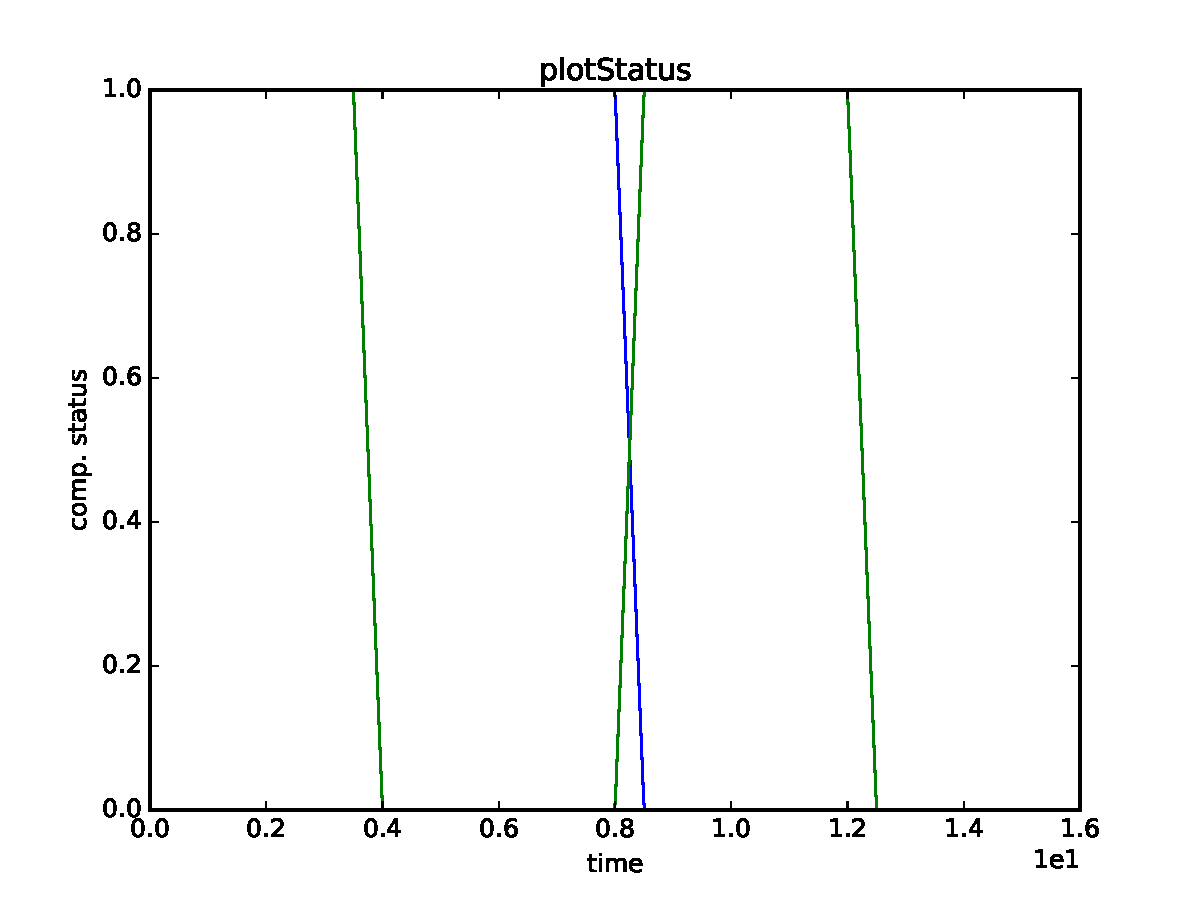
\includegraphics[scale=0.5]{1-plotStatus_line-line.pdf}}
    \caption{Temporal profile of the status for component A (blue line) and C (green line).}
    \label{fig:plotStatus_line-line}
\end{figure}

\begin{figure}
    \centering
    \centerline{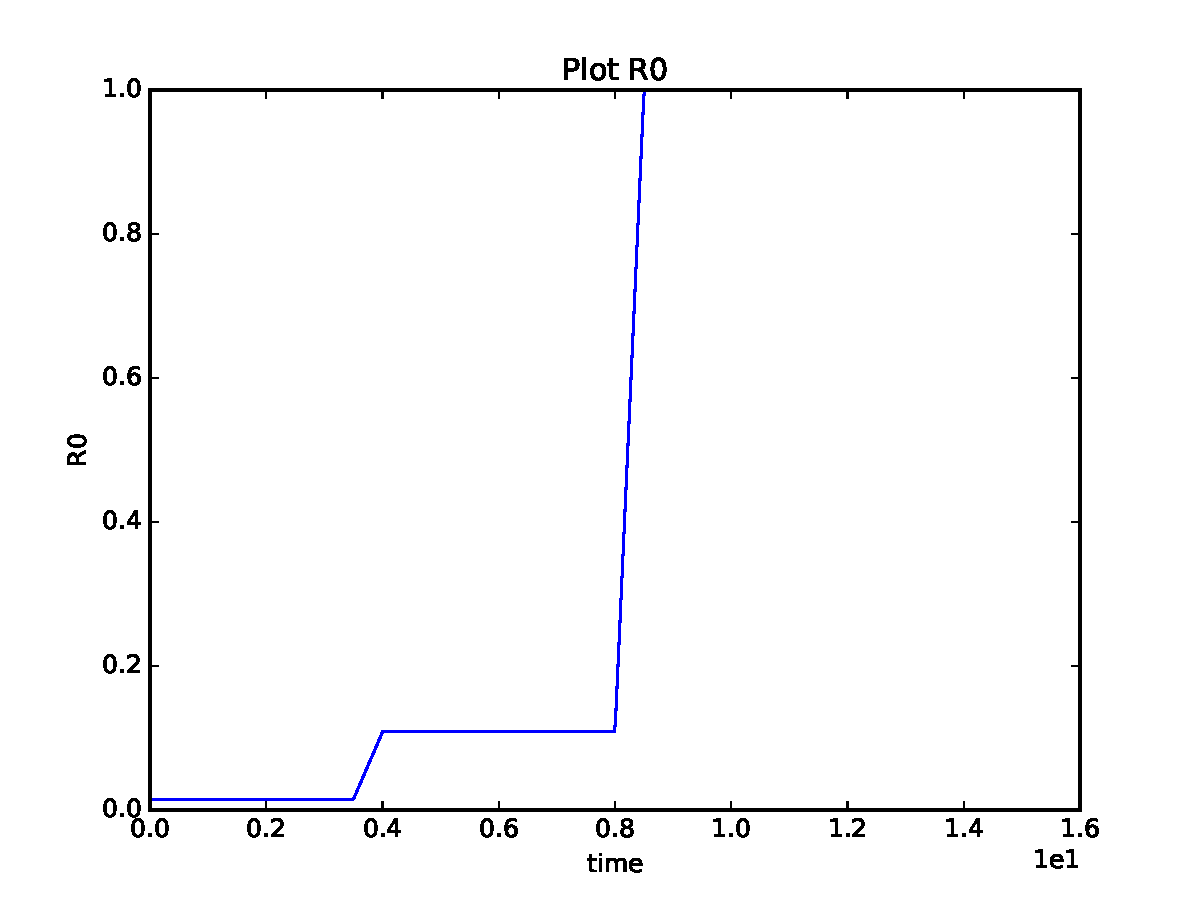
\includegraphics[scale=0.5]{1-plotR0_line.pdf}}
    \caption{Temporal profile for system failure probability.}
    \label{fig:plotR0_line}
\end{figure}

\begin{figure}
    \centering
    \centerline{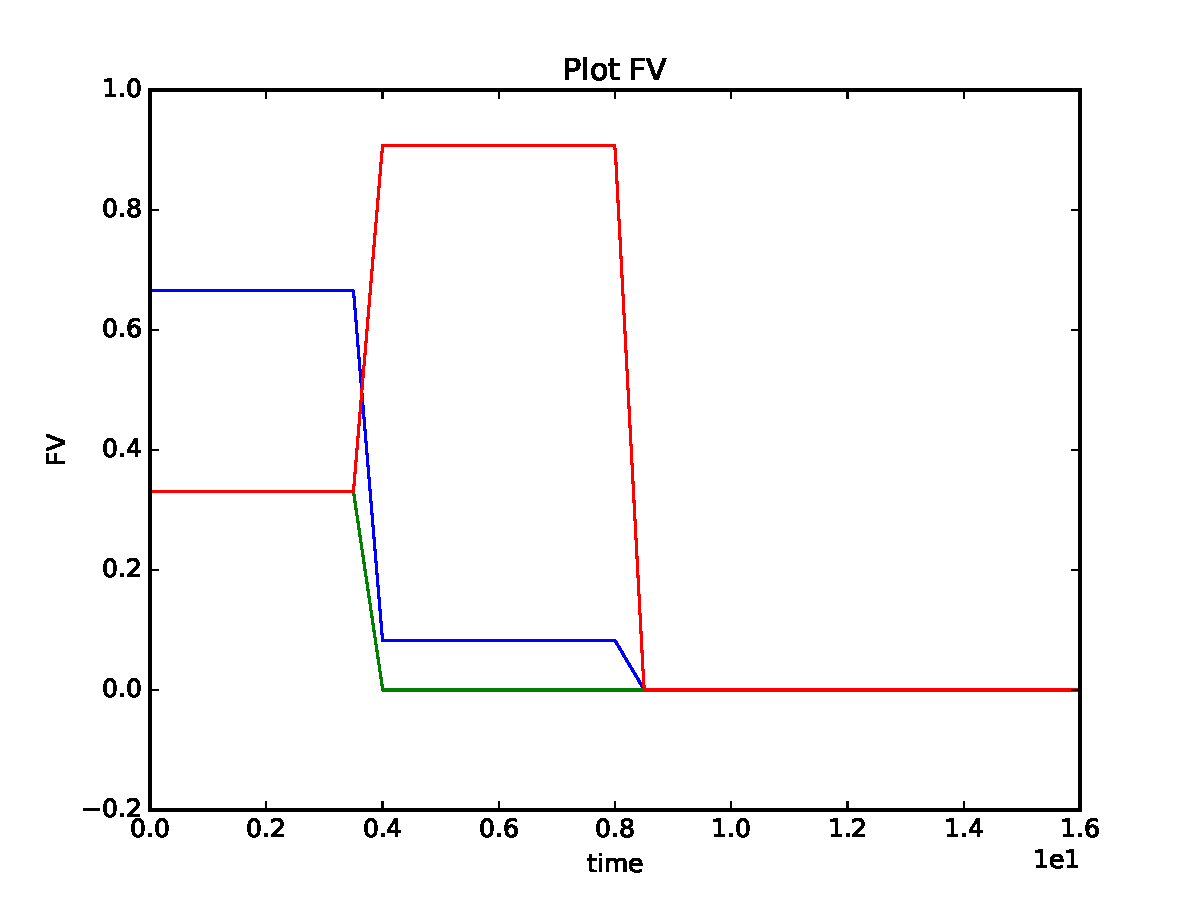
\includegraphics[scale=0.5]{1-plotFV_line-line-line.pdf}}
    \caption{FV profile for components B (green line), A (blue line) and C (red line).}
    \label{fig:plotFV_line-line-line}
\end{figure}



\section{New RIMs in a Dynamic PRA Context}
\label{sec:newRIM}

Note that the RIMs described so far are tight to a binary logic of the outcome 
variable (e.g., OK vs. CD). Dynamic PRA approaches typically generate a continuous 
value of the outcome variables (e.g., peak clad temperature - $PCT$). 
In our application (see previous sections) we typically convert $PCT$ to a discrete 
one as follows:
\begin{itemize}
  \item $PCT>2200 F$: outcome = CD
  \item $PCT<2200 F$: outcome = OK
\end{itemize}
  
Given the different structure of the approach used in this paper to solve a PRA 
problem (i.e., Dynamic instead of classical PRA), the reader might think that a different 
set of RIMs should/could be developed in order to capture the nature of the problem 
solved using Dynamic PRA.
As a starting point, it would worth investigating the nominal probabilistic distribution 
(pdf) of PCT with the one obtained when reliability of each basic event (sampled parameter) 
is 0.0 or 1.0. So now we can indicate:
\begin{itemize}
  \item $pdf_0 (T)$: nominal pdf of PCT
  \item $pdf_i^-(T)$: pdf of PCT associated to basic event $i$ assuming basic event is perfectly 
        reliable
  \item $pdf_i^+(T)$: pdf of PCT associated to basic event $i$ assuming basic event has failed
\end{itemize}

An example is shown below for a hypothetical case where obtained $pdf_0(T)$ is indicated 
using an histogram while the limit value for PCT is shown using the red line passing at 2200 F.
In order to make a connection to what has been presented in the previous section, note that by 
looking at Fig.~\ref{fig:margin0}:
\begin{equation}
  R_0 = \int_{2200}^\infty \! pdf_0(T) \, dT
  \label{eq:R0}
\end{equation}

As part of the RISMC analysis, the user might want to supplement the results obtained in the 
previous section with the information associated to a more effective margin analysis.
In particular, of interest for RISMC applications is (see Fig.~\ref{fig:margin0}) the concept of margin:
\begin{equation}
  margin= 2200-PCT \text{ given } PCT<2200
  \label{eq:margin}
\end{equation}

\begin{figure}
  \centering
  \begin{subfigure}{.5\textwidth}
    \centering
    \centerline{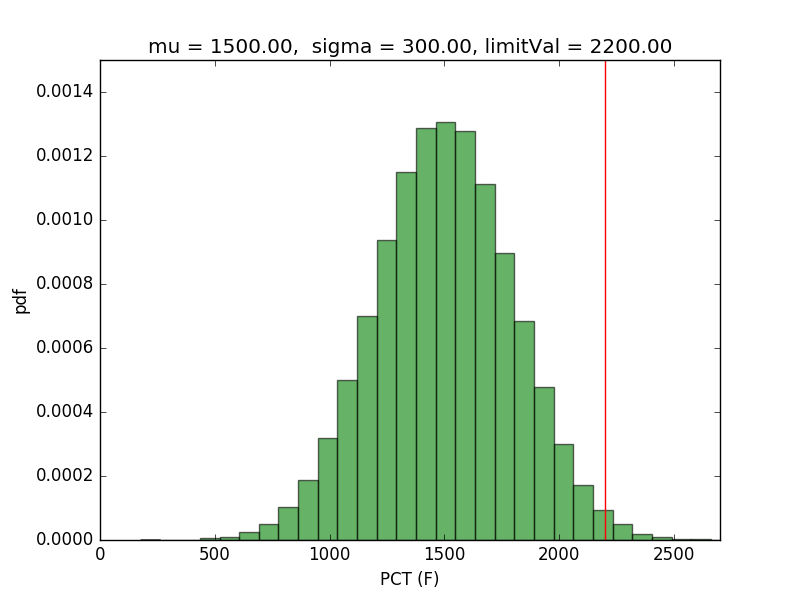
\includegraphics[scale=0.3]{pdf0.png}}
  \end{subfigure}%
  \begin{subfigure}{.5\textwidth}
    \centering
    \centerline{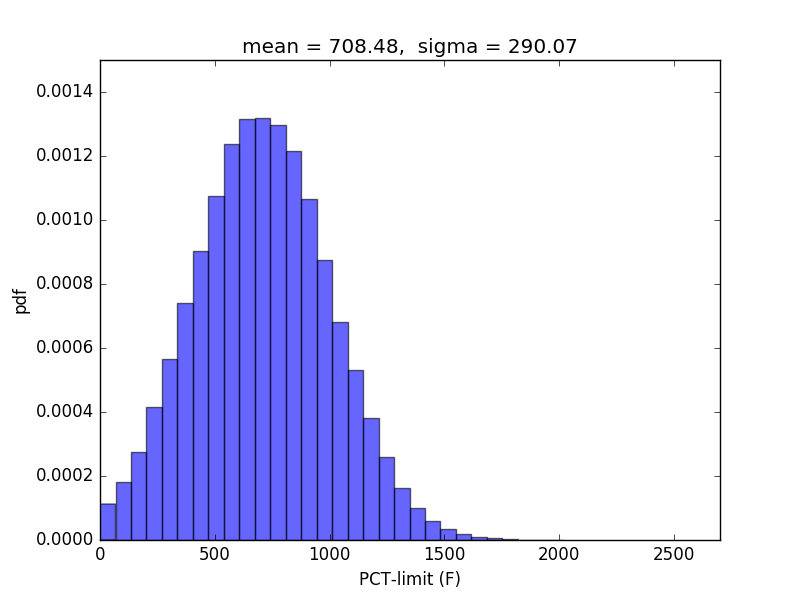
\includegraphics[scale=0.3]{margin0.png}}
  \end{subfigure}
  \caption{Plot of a hypothetical $pdf_0(T)$ (left) and its associated margin $margin_0$ (right).}
  \label{fig:margin0}
\end{figure}
 
Using the same philosophy indicated in the previous section for classical RIMs, we want 
to determine:
\begin{itemize}
  \item $margin_0$: pdf of the variable $2200-PCT$ given that $PCT<2200$
  \item $margin_i^-$: pdf of the variable $2200-PCT$ given that $PCT<2200$ for basic 
                      event $i$ assuming it is perfectly reliable
  \item $margin_i^+$: pdf of the variable $2200-PCT$ given that $PCT<2200$ for basic event 
                      $i$ when its assumed to be failed
\end{itemize}

Note now that $margin_0$, $margin_i^-$ and $margin_i^+$ are now pdfs and not numerical values. 
Hence, now the challenge arises on how to compare two pdfs:
\begin{itemize}
  \item $margin_0$ vs. $margin_i^-$
  \item $margin_0$ vs. $margin_i^+$
\end{itemize}

\begin{figure}
  \begin{subfigure}{.5\linewidth}
  \centering
  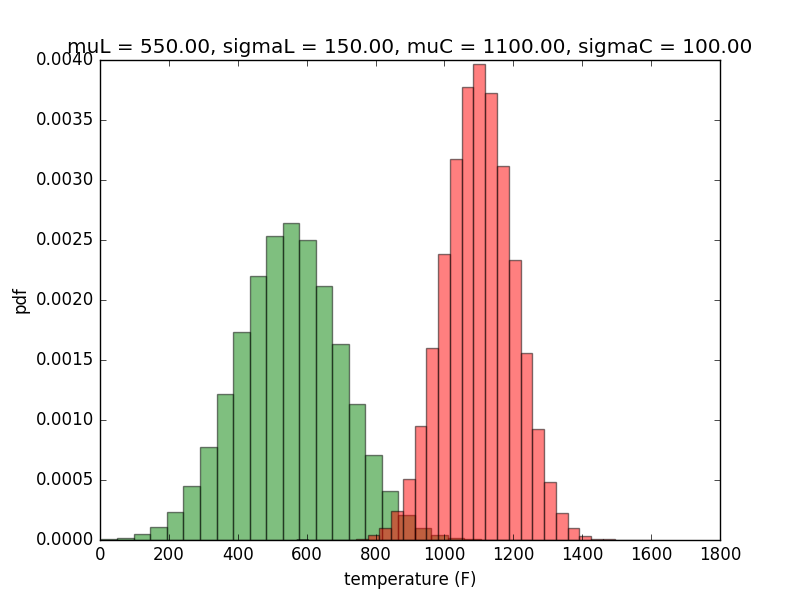
\includegraphics[scale=.3]{dist_dist_1.png}
  \end{subfigure}%
  \begin{subfigure}{.5\linewidth}
  \centering
  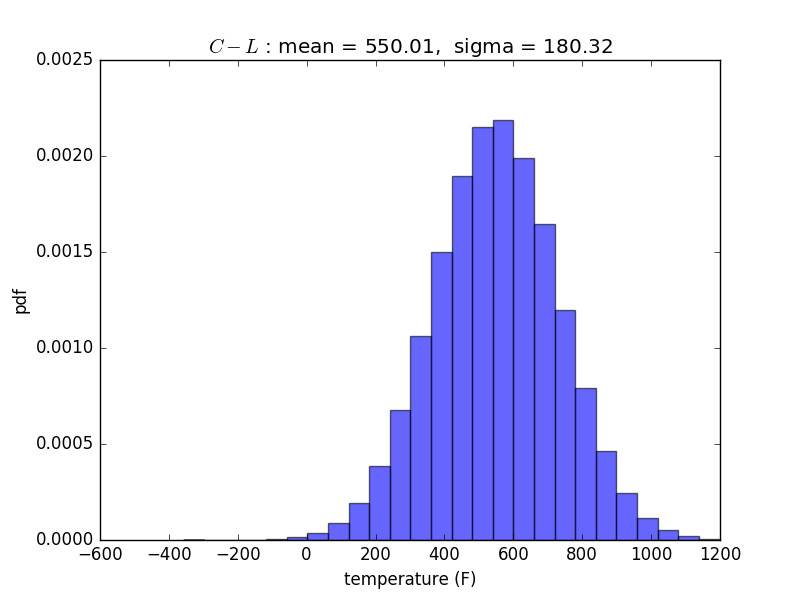
\includegraphics[scale=.3]{dist_dist_2.png}
  \end{subfigure}\\[1ex]
  \begin{subfigure}{\linewidth}
  \centering
  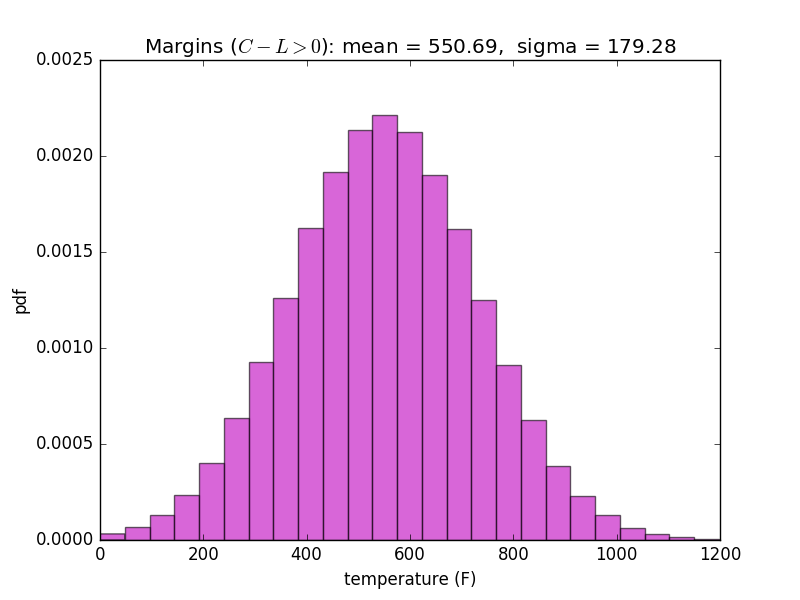
\includegraphics[scale=.3]{dist_dist_3.png}
  \end{subfigure}
  \caption{Plot of the pdfs for $PCT$ (green) and $CFT$ (red) (top left), 
           Plot of the pdf of the variable $CFT-PCT$ (top right) and 
           Plot of the pdf of the margin, i.e., $CFT-PCT>0$ (bottom).}
  \label{fig:dist_dist}
\end{figure}

Assume two pdfs are given: $pdf_1(x)$ and $pdf_2(x)$. Few approaches can be followed: Z-test or 
Kolmogorov–Smirnov test. 
In the first approach (Z-test), the following variable $Z$ is computed:
\begin{equation}
  Z_{1,2} = \frac{mean(pdf_1)-mean(pdf_2)}{\sqrt{std\_dev^2 (pdf_1)-std\_dev^2(pdf_2)}} 
  \label{eq:Ztest}
\end{equation}
where:
\begin{itemize}
  \item $mean(pdf)$ correspond to the mean of $pdf(x)$ 
  \item $std\_dev(pdf)$ correspond to the standard deviation of $pdf(x)$ 
\end{itemize}

In the second approach (Kolmogorov–Smirnov test~\cite{}), instead of the pdf, the cumulative 
distribution functions (pdf) are considered: $cdf_1(x)$ and $cdf_2(x)$. 
In particular, the Kolmogorov-Smirnov statistic is calculated as:
\begin{equation}
  Z_{1,2} = \sup_{x} (cdf_1(x) - cdf_2(x))
  \label{eq:Kolmogorov-Smirnov}
\end{equation}

Note that so far we have imposed clad failure temperature ($CFT$) to be a fixed value, 
i.e., 2200 F. 
In many RISMC applications $CFT$ is no longer a numerical value but it can be un uncertain 
parameter, i.e., a pdf is associated to CDF: $pdf(T)$. 
This link goes back to the original logo of RISMC where a pdf for ``load'' and ``capacity'' 
(see Fig.~\ref{}).
A new definition of margin can be then defined:

\begin{equation}
  margin=(CFT-PCT) \text{ given } (CFT-PCT>0)
  \label{eq:new margin}
\end{equation}

From here, once the pdf associated to the margin variable is determined it is possible 
to employ either the Z-tests or the Kolmogorov–Smirnov test in order to measure how this pdf 
changes when each basic event is considered perfectly reliable or failed. 

\section{Conclusions}
\label{sec:conclusions}
In this paper, a newly developed capability of the RAVEN code has been shown. Through the Ensemble-Model entity, RAVEN is able to combine multiple models (i.e. Simulation Codes, Reduced Order Models, etc.), constructing a pipe network in order to transfer information among them. The addition of the Picard’s iteration scheme lets the user solving combinations of models that resolve in non-linear systems. 
The paper shows the early results for implementation of an ensemble approach for the coupling of surrogate models representing a multi-physics problem. While this is an initial implementation, the developed structure seems to support current needs and will be eventually extended in the future in order to couple codes whose input/output space is represented by high-density fields (e.g. temperature profiles in each nodal kinetic zones, etc.). This capability builds a complex system representation, even when the original models were not coupled, but just coupled their surrogate. Two applications are relevant for reliability analysis: (1) the possibility to build surrogate representation of a complex system, starting from libraries of surrogate models for each component, and (2) software implementation present during the first stage of surrogate model coupling when responses are high-density fields. 
The Ensemble-Model capability in RAVEN is currently used to couple a fuel performance code (Bison) and the T-H system code RELAP5 in order to analyze LOCA scenarios.ion.

\section*{Appendix A: Analytical Results}
\label{sec:appendixA}

\subsection*{Example 1}
\label{sec:example1Anal}

For the system described in Section~\ref{sec:example1} we have the following

\begin{align} 
  R_0   &= p_A + p_B p_C - p_A p_B p_C = 0.01495   \\
  R_A^- &= p_B p_C = 0.005  \\
  R_A^+ &= 1.0  \\
  R_B^- &= p_A = 0.01  \\
  R_B^+ &= p_A + p_C - p_A p_C = 0.109  \\
  R_C^- &= p_A = 0.01 \\
  R_C^+ &= p_A + p_B - p_A p_B = 0.0595  
\end{align}

Thus:
\begin{align} 
  FV_A &= \frac{R_0-R_A^-}{R_0} = 0.665552 \\
  FV_B &= \frac{R_0-R_B^-}{R_0} = 0.331104 \\
  FV_C &= \frac{R_0-R_C^-}{R_0} = 0.331104    
\end{align}
and:
\begin{align} 
  RAW_A &= \frac{R_i^+}{R_0} = 66.88963 \\
  RAW_B &= \frac{R_i^+}{R_0} = 7.29097 \\
  RAW_C &= \frac{R_i^+}{R_0} = 3.97993    
\end{align}

\subsection*{Example 2}
\label{sec:example2Anal}

We can solve the system described in Section~\ref{sec:example2} using reliability
block diagrams (see Fig.~\ref{fig:example2RBB}).

\begin{figure}
    \centering
    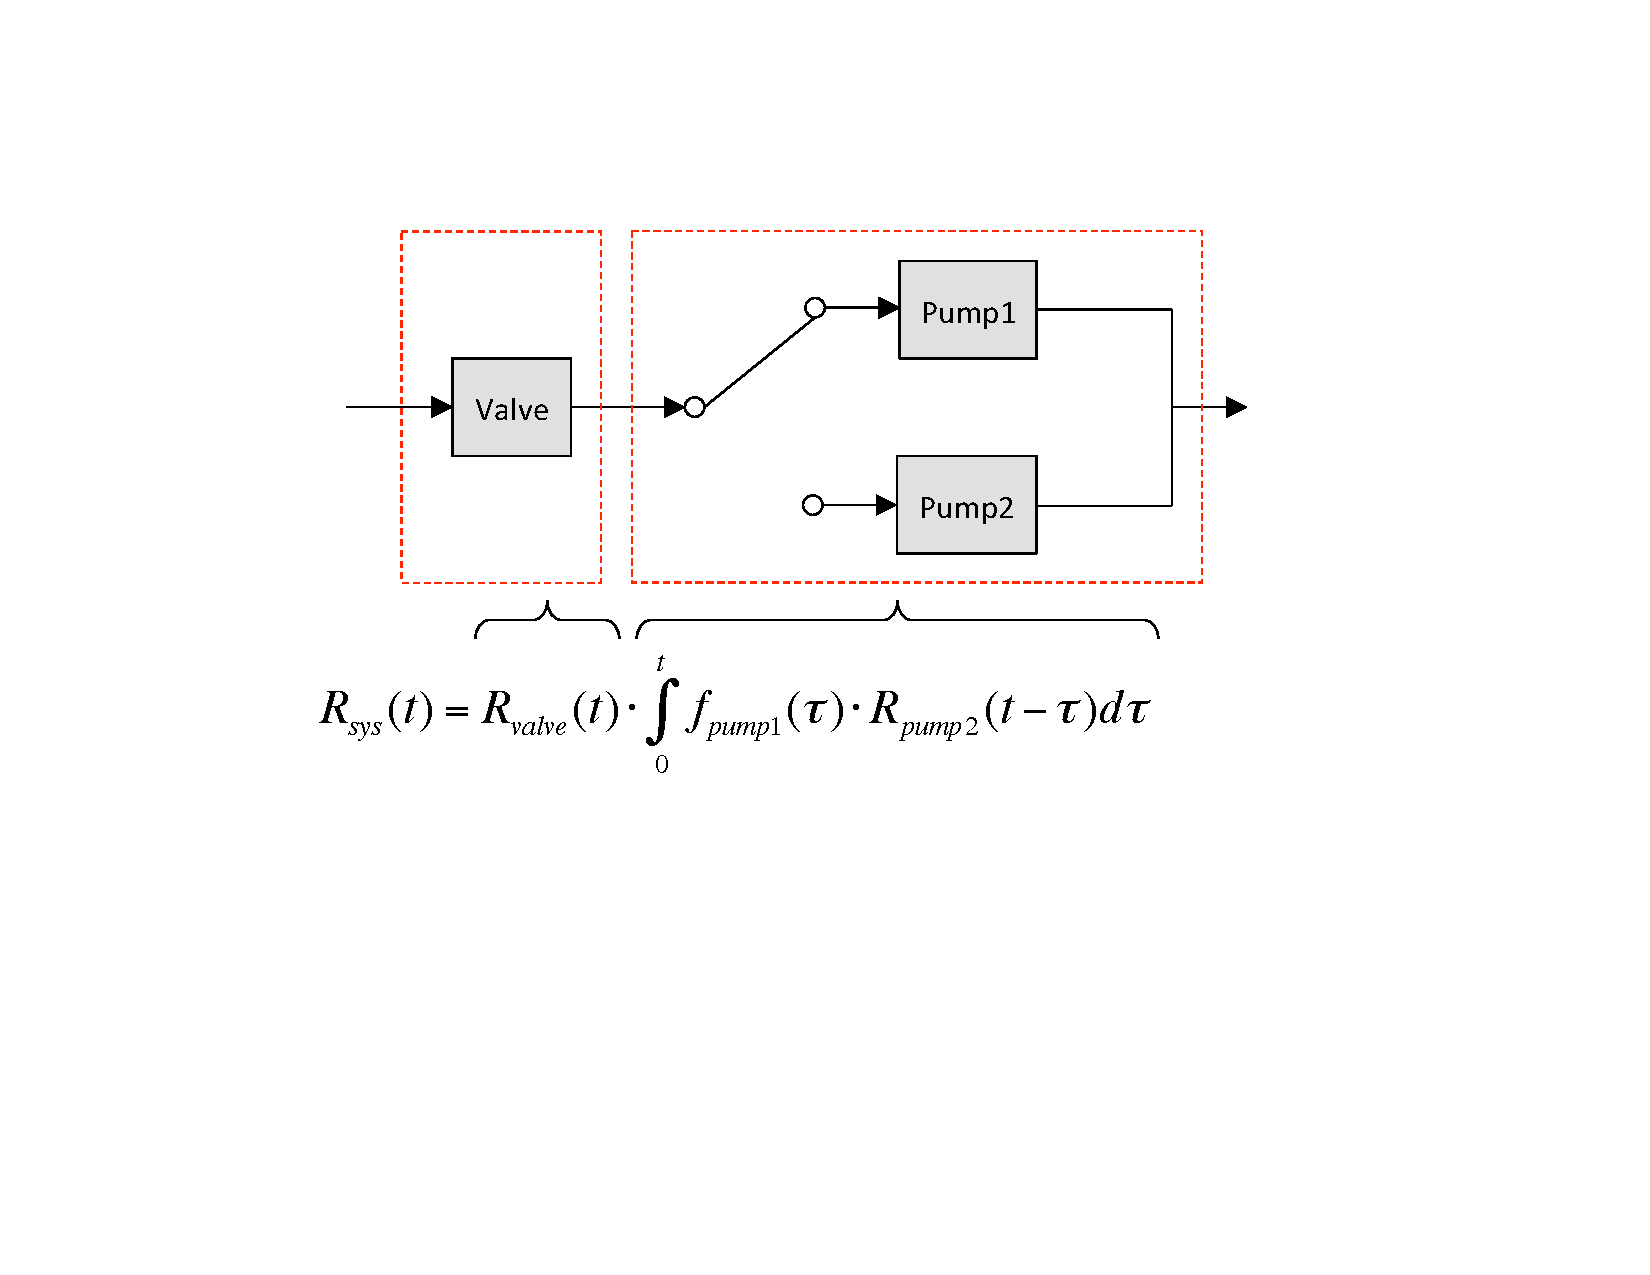
\includegraphics[scale=0.5]{blocks.pdf}
    \caption{Reliability block diagrams for Example 2 (see Section~\ref{sec:example2}).}
    \label{fig:example2RBB}
\end{figure}

Thus time dependent reliability of the system $R_sys(t)$ as function of time $t$:
\begin{equation}
  R_{sys}(t) = R_{valve}(t) \int_0^t f_{pump1}(\tau) R_{pump2}(t-\tau) d\tau
\end{equation}
where:
\begin{itemize}
  \item $R_{valve}(t) = e^{-\lambda_{valve} t}$
  \item $f_{pump1}(t) = \lambda_{pump1} e^{-\lambda_1 t}$
  \item $R_{pump2}(t) = e^{-\lambda_{pump2} t}$
\end{itemize}

It can be shown that if $\lambda_{pump1} = \lambda_{pump2} = \bar{\lambda}$:
\begin{equation}
  R_{sys}(t) = e^{-\lambda_{valve} t} [ e^{-\bar{\lambda}} (1+\bar{\lambda} t) ]
\end{equation}

For this system we have the following for a mission time $T=24$ hours:
\begin{align} 
  & R_0         = 1.0 - R_{sys}(T) = 0.85063876  \\
  & R_{valve}^- = 1.0 - [ e^{-\bar{\lambda} T} (1+\bar{\lambda} T) ] = 0.593994129 \\
  & R_{valve}^+ = 1.0  \\
  & R_{pump1}^- = 1.0 - R_{valve}(T) = 0.6321205  \\
  & R_{pump1}^+ = 1.0 - R_{valve}(T) R_{pump2}(T) = 0.95021292 \\
  & R_{pump2}^- = R_{pump1}^- = 0.6321205 \\
  & R_{pump2}^+ = R_{pump1}^+ = 0.95021292
\end{align}

\subsection*{Example 3}
\label{sec:example3Anal}

We can solve the system described in Section~\ref{sec:example2} using again reliability
block diagrams.
Thus time dependent reliability of the system $R_sys(t)$ as function of time $t$:
\begin{equation}
  R_{sys}(t) = R_{valve}(t) R_{2oo3}(t)
\end{equation}
where $R_{2oo3}(t)$ represents reliability of a set of three identical components 
in a 2 out of 3 (2oo3) configuration. 

It can be shown that if 
$\lambda_{pump1} = \lambda_{pump2} = \lambda_{pump3} = \bar{\lambda}$
(thus $R_{pump1}(t) = R_{pump2}(t) = R_{pump3}(t) = \bar{R}(t) = e^{- \bar{\lambda} t}$)
then $R_{2oo3}(t)$ can be written as
\begin{equation}
  R_{2oo3}(t) = \sum\limits_{n=2}^3 \binom{3}{n} \bar{R}(t)^n [1-\bar{R}(t)]^{3-n}
              = 3 e^{- 2 \bar{\lambda} t} (1 - e^{- \bar{\lambda} t}) + e^{- 3 \bar{\lambda} t}
\end{equation}

For this system we have the following for a mission time $T=24$ hours:
\begin{align} 
  & R_0         = 1.0 - R_{sys}(T) = 0.981609917 \\
  & R_{valve}^- = 1.0 - R_{2oo3}(T) = 0.95001058 \\
  & R_{valve}^+ = 1.0 \\
  & R_{pump1}^- = 1.0 - R_{1oo2}(T) R_{valve}(T) = 0.907163789\\
  & R_{pump1}^+ = 1.0 - R_{valve}(T) \bar{R}(t)^2 = 0.993262051\\
  & R_{pump2}^- = R_{pump1}^- \\
  & R_{pump2}^+ = R_{pump1}^+ \\
  & R_{pump3}^- = R_{pump1}^- \\
  & R_{pump3}^+ = R_{pump1}^+ 
\end{align}
where $R_{1oo2}(t)$ represents reliability of a set of two identical components 
in a 1 out of 2 (1oo2) configuration:

\begin{equation}
  R_{1oo2}(t) = \sum\limits_{n=1}^2 \binom{2}{n} \bar{R}(t)^n [1-\bar{R}(t)]^{2-n}
              = 2 e^{- \bar{\lambda} t} (1 - e^{- \bar{\lambda} t}) + e^{- 2 \bar{\lambda} t}
\end{equation}


\section*{References}

\bibliography{main}

\end{document}